%%%%%%%%%%%%%%%%%%%%%%%%%%%%%%%%%%%%%%%%%
% Short Sectioned Assignment
% LaTeX Template
% Version 1.0 (5/5/12)
%
% This template has been downloaded from:
% http://www.LaTeXTemplates.com
%
% Original author:
% Frits Wenneker (http://www.howtotex.com)
%
% License:
% CC BY-NC-SA 3.0 (http://creativecommons.org/licenses/by-nc-sa/3.0/)
%
%%%%%%%%%%%%%%%%%%%%%%%%%%%%%%%%%%%%%%%%%

%----------------------------------------------------------------------------------------
%  PACKAGES AND OTHER DOCUMENT CONFIGURATIONS
%----------------------------------------------------------------------------------------

\documentclass[norsk]{article} % A4 paper and 11pt font size

\usepackage[T1]{fontenc} % Use 8-bit encoding that has 256 glyphs
\usepackage{fourier} % Use the Adobe Utopia font for the document - comment this line to return to the LaTeX default
\usepackage[english]{babel} % English language/hyphenation
\usepackage{amsmath,amsfonts,amsthm} % Math packages

% Added by Joergen %---------------------------------------------------------------------
%\usepackage{cleveref}
\usepackage{soul}

\usepackage{listings}
\usepackage{xcolor}
\newcommand{\textcolordummy}[2]{#2}

\definecolor{mygray}{rgb}{0.4,0.4,0.4}
%\definecolor{mycyan}{rgb}{0,0.8,0.6}
\definecolor{mygreen1}{rgb}{0.3,0.6,0.3}
\definecolor{mygreen2}{rgb}{0,0.4,0.1}
\definecolor{myorange}{rgb}{1.0,0.4,0}

\lstset{language=C++,
                basicstyle={\color{black}\footnotesize\ttfamily\let\textcolor\textcolordummy},
                %identifierstyle=\color{green},
                keywordstyle={\color{blue}\footnotesize\ttfamily\let\textcolor\textcolordummy},
                %keywordstyle={\color{blue}\footnotesize\ttfamily\let\textcolor\textcolordummy},
                directivestyle={\color{mygreen1}},
                emph={int,char,double,float,unsigned},
                emphstyle={\color{mygreen2}},
                %
                stringstyle={\color{myorange}\footnotesize\ttfamily\let\textcolor\textcolordummy},
                %stringstyle={\color{orange}\footnotesize\ttfamily\let\textcolor\textcolordummy},
                commentstyle={\color{mygray}\footnotesize\ttfamily\let\textcolor\textcolordummy},
                morecomment=[l][\color{magenta}]{\#}
                %
                showspaces=false,  
                showstringspaces=false, 
                showtabs=false,
                extendedchars=true,
                frame=single,  
}
\lstdefinestyle{FormattedNumber}{%
    literate={0}{{\textcolor{red}{0}}}{1}%
             {1}{{\textcolor{red}{1}}}{1}%
             {2}{{\textcolor{red}{2}}}{1}%
             {3}{{\textcolor{red}{3}}}{1}%
             {4}{{\textcolor{red}{4}}}{1}%
             {5}{{\textcolor{red}{5}}}{1}%
             {6}{{\textcolor{red}{6}}}{1}%
             {7}{{\textcolor{red}{7}}}{1}%
             {8}{{\textcolor{red}{8}}}{1}%
             {9}{{\textcolor{red}{9}}}{1}%
             {.0}{{\textcolor{red}{.0}}}{2}% Following is to ensure that only periods
             {.1}{{\textcolor{red}{.1}}}{2}% followed by a digit are changed.
             {.2}{{\textcolor{red}{.2}}}{2}%
             {.3}{{\textcolor{red}{.3}}}{2}%
             {.4}{{\textcolor{red}{.4}}}{2}%
             {.5}{{\textcolor{red}{.5}}}{2}%
             {.6}{{\textcolor{red}{.6}}}{2}%
             {.7}{{\textcolor{red}{.7}}}{2}%
             {.8}{{\textcolor{red}{.8}}}{2}%
             {.9}{{\textcolor{red}{.9}}}{2}%
             ,
   basicstyle=\footnotesize\ttfamily,%  Optional to use this
}


% Added by Haavard %---------------------------------------------------------------------
\usepackage[utf8]{inputenc} % Norwegian letters
\usepackage{fullpage}
\usepackage{subcaption}
\usepackage[font={small, it}]{caption} % captions on figures and tables
\usepackage{graphicx}
\usepackage{color}
\usepackage{hyperref} % Use \autoref{ and \nameref{
\hypersetup{backref,
colorlinks=true,
breaklinks=true,
%hidelinks, %uncomment to make links black
linkcolor=blue,
urlcolor=blue,
citecolor=blue
}
\usepackage[all]{hypcap} % Makes hyperref jup to top of pictures and tables
% --------------------------------------------------------------------------------------

\usepackage{lipsum} % Used for inserting dummy 'Lorem ipsum' text into the template

\usepackage{sectsty} % Allows customizing section commands
\allsectionsfont{\centering \normalfont\scshape} % Make all sections centered, the default font and small caps

\usepackage{fancyhdr} % Custom headers and footers
\pagestyle{fancyplain} % Makes all pages in the document conform to the custom headers and footers
\fancyhead{} % No page header - if you want one, create it in the same way as the footers below
\fancyfoot[L]{} % Empty left footer
\fancyfoot[C]{} % Empty center footer
\fancyfoot[R]{\thepage} % Page numbering for right footer
\renewcommand{\headrulewidth}{0pt} % Remove header underlines
\renewcommand{\footrulewidth}{0pt} % Remove footer underlines
\setlength{\headheight}{13.6pt} % Customize the height of the header

\numberwithin{equation}{section} % Number equations within sections (i.e. 1.1, 1.2, 2.1, 2.2 instead of 1, 2, 3, 4)
\numberwithin{figure}{section} % Number figures within sections (i.e. 1.1, 1.2, 2.1, 2.2 instead of 1, 2, 3, 4)
\numberwithin{table}{section} % Number tables within sections (i.e. 1.1, 1.2, 2.1, 2.2 instead of 1, 2, 3, 4)

\setlength\parindent{0pt} % Removes all indentation from paragraphs - comment this line for an assignment with lots of text

%----------------------------------------------------------------------------------------
%  TITLE SECTION
%----------------------------------------------------------------------------------------

\newcommand{\horrule}[1]{\rule{\linewidth}{#1}} % Create horizontal rule command with 1 argument of height

\title{  
\normalfont \normalsize 
\textsc{NTNU 2015} \\ [25pt] % Your university, school and/or department name(s)
\horrule{0.5pt} \\[0.4cm] % Thin top horizontal rule
\huge Project Notes\\ % The assignment title
\horrule{2pt} \\[0.5cm] % Thick bottom horizontal rule
}

\author{Jørgen Vågan \\ Supervisor: Ingve Simonsen} % Your name

\date{\normalsize\today} % Today's date or a custom date


\begin{document}


\maketitle % Print the title

%----------------------------------------------------------------------------------------
%  Text Body:
%----------------------------------------------------------------------------------------

%\listoftodos{}

\abstract{ Abstract..
abstract.}

\newpage
\section{Additional Theory}

\subsection{Complex permittivity and refractive index (From wikipedia) don't use, LACKING REFERENCES!}
Complex electric permittivity:
\begin{align}
   \hat{\varepsilon}_r(\omega) = \frac{\hat{\varepsilon} (\omega)}{\varepsilon_0}
\end{align}
where 
\begin{align}
   \hat{\varepsilon}_r(\omega) &= \varepsilon_r (\omega) + i\tilde{\varepsilon}_r (\omega) \\
                               &= \varepsilon_r (\omega) + i\frac{\sigma}{\omega\varepsilon_0} 
\end{align}
The complex refractive index $\hat{n}$ is given by 
\begin{align}
   \hat{n} = \sqrt{\hat{\varepsilon}_r},
\end{align}
when the magnetic properties are neglected ($\mu_r = 1$). 
From this, an expression for the complex refractive index $\hat{n} = n - \boldsymbol{i}\kappa$ can be found:
\begin{align}
   \hat{\varepsilon}_r &= \hat{n}^2 \\
   \varepsilon_r + \boldsymbol{i}\tilde{\varepsilon}_r &= (n + \boldsymbol{i} \kappa)^2 \\
   \varepsilon_r + \boldsymbol{i}\tilde{\varepsilon}_r &= n^2 - \kappa^2 + \boldsymbol{i}2n\kappa
\end{align}
giving
\begin{align}
   \varepsilon_r &= n^2 - \kappa^2     &\tilde{\varepsilon}_r  &= 2n\kappa.
\end{align}
Taking the absolute value or modulus of the relative permettivity
\begin{align}
   |\hat{\varepsilon}_r| &= \sqrt{ \varepsilon_r^2 + \tilde{\varepsilon}_r^2} \\
   |\hat{\varepsilon}_r| &= \sqrt{ (n^2 - \kappa^2)^2 + (2n\kappa)^2} \\
   |\hat{\varepsilon}_r|^2 &= (n^4 - 2n^2\kappa^2 + \kappa^4) + 4n^2\kappa^2 \\
   |\hat{\varepsilon}_r|^2 &= n^4 + 2n^2\kappa^2 + \kappa^4 \\
   |\hat{\varepsilon}_r|^2 &= (n^2 + \kappa^2)^2 \\
   |\hat{\varepsilon}_r| &= n^2 + \kappa^2 
\end{align}
and adding or substracting the real part of the permittivity, gives
\begin{align}
   |\hat{\varepsilon}_r| + \varepsilon_r &= (n^2 + \kappa^2) + (n^2 - \kappa^2) = 2n^2\\
   |\hat{\varepsilon}_r| - \varepsilon_r &= (n^2 + \kappa^2) - (n^2 - \kappa^2) = 2\kappa^2.
\end{align}
Refomulating the expression gives the real and imaginary parts of $\hat{n}$
\begin{align}
   n      &= \sqrt{ \frac{|\hat{\varepsilon}_r| + \varepsilon_r}{2}} 
           = \sqrt{ \frac{|\hat{\varepsilon}| + \varepsilon}{2\varepsilon_0}}\\
   \kappa &= \sqrt{ \frac{|\hat{\varepsilon}_r| - \varepsilon_r}{2}} 
           = \sqrt{ \frac{|\hat{\varepsilon}| - \varepsilon}{2\varepsilon_0}}
\end{align}


\subsection{Polarizability. Don't use, LACKING REFERENCES}
When a neutral atom is placed in an electric field $\boldsymbol{E}$, the field tries to rip the
atom apart by pushing the nucleus in the direction of the field and the electrons in the opposite direction.
Because of the attraction between the positive and negative charge within the atom, an equilibrium displacement
of the electrons compared to the nucleus is achieved, leaving the atom polarized and giving it a
dipole moment. The dipole moment can be approximated by
\begin{align}
   \boldsymbol{p} = \alpha \boldsymbol{E},
\end{align}
where $\alpha$ is the atomic polarizability and may depend on the detailed structure of the atom.
For more complicated situations, like an asymmetrical molecule, the gained dipole moment of the 
molecule does not necessarily have to be in the same direction as the applied electric field.
In such a case, the scalar polarizability in the expression above is replaced by a polarizability tensor
\begin{align}
   \boldsymbol{\alpha} = 
\begin{bmatrix}
   \alpha_{xx}   &   \alpha_{xy}  &  \alpha_{xz}  \\
   \alpha_{yx}   &   \alpha_{yy}  &  \alpha_{yz}  \\
   \alpha_{zx}   &   \alpha_{zy}  &  \alpha_{zz} 
\end{bmatrix}
.
\end{align}
In this way, an applied eletric field induces many dipole moments in a material. In addition,
any polar molecules will be subject to a torque, aligning it to the direction of the field.
These two mechanisms leads to the polarization $\boldsymbol{P}$ of the material
\begin{align}
   \boldsymbol{P} = \text{dipole moment per unit volume} = \varepsilon_0 \chi_e \boldsymbol{E}.
\end{align}
In the above expression, there has been assumed a linear dielectric media, where $\chi_e$ is the electric 
susceptibility and depends on the microscopic structure of the material, in addition to the external 
temperature (\cite{Griffiths},p.160-166, 179)

\subsection{The electric potential, Laplace's equation and the Uniqueness Theorem}
The usual task of electrostatics is to ompute the electric field $\boldsymbol{E}$ given a 
stationary charge distribution $\rho{\boldsymbol{r}}$
\begin{align}
   \boldsymbol{E}(\boldsymbol{r}) 
   &= \frac{1}{4 \pi \varepsilon_0} \int \frac{\boldsymbol{\hat{d}}(\boldsymbol{r'})}
                                              {d(\boldsymbol{r'})^2} 
                                                            \rho(\boldsymbol{r'}) d\!\boldsymbol{r'} 
                                                            \\
   &= \frac{1}{4 \pi \varepsilon_0} \int \frac{\boldsymbol{r} - \boldsymbol{r'}}
                                              {\big|\boldsymbol{r} - \boldsymbol{r'}\big|^3} 
                                                           \rho(\boldsymbol{r'}) d\!\boldsymbol{r'}.
\end{align}
However, it is usually simpler to calculate the potential
\begin{align}
   \label{electricPotential}
   V(\boldsymbol{r}) 
   &= \frac{1}{4 \pi \varepsilon_0} \int \frac{1}{\big|\boldsymbol{r} - \boldsymbol{r'}\big|} 
                                                           \rho(\boldsymbol{r'}) d\!\boldsymbol{r'}
\end{align}
first and then calculate the electric field from
\begin{align}
   \boldsymbol{E} = - \nabla V.
\end{align}
This might in some situations, where do do not necessarily know $\rho$ but only the total amount of 
charge, also be to tough to handle analytically. In situations like these it is better to use
Poisson's equation
\begin{align}
   \label{poisson}
   \nabla^2 V= - \frac{1}{\varepsilon_o} \rho,
\end{align}
which together with appropriate boundary conditions, is equivalent to Eq.\eqref{electricPotential}.
Very often, we are interested in finding the potential containing no charge (because the charge is 
located on the outside of our region of interest. In such cases Eq. \eqref{poisson} reduces to
Laplace's equation (\cite{Griffiths}, p.110-111)
\begin{align}
   \label{laplace}
   \nabla^2 V = 0.
\end{align}
According to the \textit{Uniqueness Theorems}, the solution to Laplace's equation is uniquely 
determined in some volume if the potential is specified on the boundary of the volume. This
easily extends to Poisson's equation by further requiring, in addition to the 
potential on the boundary, that the charge distribution throughout the region is known.
\\
\\
When considering conductors, charge are allowed to move freely and  might start to rearrange themselves,
leading to the \textit{Second uniqueness theorem}, which states that the potential in a given volume,
surrounded by conductors is uniquely determined if the total charge on each conductor is given.
\\
\\
The uniqueness theorem grants an enlarged mathematical freedom in the approach of finding the potential
of a region of space. This is because the boundary uniquely determines the potential in the region enclosed
region and any approach giving the correct boundary conditions would give you the correct potential 
function through Laplace's equation Eq. \eqref{laplace}. This allows the use of tricks, like for example
the classical \textit{method of images} (\cite{Griffiths}, p.116-121).
%SOME EXTRA STUFF:
%\textbf{D'Alembert Operator $\square$}
%\begin{align*}
  %\square  &= \partial ^{\mu} \partial _{\mu}
   %\\
           %&= \frac{1}{c^2} \frac{\partial ^2}{\partial t^2} 
               %- \frac{\partial ^2}{\partial x^2} 
               %- \frac{\partial ^2}{\partial y^2} 
               %- \frac{\partial ^2}{\partial z^2} 
   %\\
           %&= \frac{1}{c^2} \frac{\partial ^2}{\partial t^2} - \nabla ^2
%\end{align*}

%\textbf{Lorentz Gauge:} \\
%For Lorentz invariance, convenient to choose the Lorenz gauge:
%\begin{align*}
   %\square \vec{A} = \Bigg[ \frac{1}{c^2} \frac{\partial ^2}{\partial t^2} - \nabla ^2 \Bigg] \vec{A} = \mu_0 \vec{J}
%\end{align*}
%\begin{align*}
   %\square \phi = \Bigg[ \frac{1}{c^2} \frac{\partial ^2}{\partial t^2} - \nabla ^2 \Bigg] \phi = \frac{\rho}{\epsilon _0}
%\end{align*}

\section{Basic Theory}
\subsection{The electric potential, Laplace's equation and the Uniqueness Theorem}
The usual task of electrostatics is to compute the electric field $\boldsymbol{E}$ given a 
stationary electric charge distribution $\rho_E{\boldsymbol{r'}}$
\begin{align}
   \label{electricField}
   \boldsymbol{E}(\boldsymbol{r}) 
   %&= \frac{1}{4 \pi \varepsilon_0} \int \frac{\boldsymbol{\hat{d}}(\boldsymbol{r'})}
                                              %{d(\boldsymbol{r'})^2} 
                                                            %\rho(\boldsymbol{r'}) d\!\boldsymbol{r'} 
                                                            %\\
   &= \frac{1}{4 \pi \varepsilon_0} \int \frac{\boldsymbol{r} - \boldsymbol{r'}}
                                              {\big|\boldsymbol{r} - \boldsymbol{r'}\big|^3} 
                                                           \rho(\boldsymbol{r'}) d\!\boldsymbol{r'}.
\end{align}
The notation for Eq.\eqref{electricField} can be shown in Figure \ref{fig:electricField}
and $\varepsilon_0 = 8.85 \cdot 10 ^{-12} \text{C}^2/\text{Nm}^2$ is the permittivity of free space
\cite[.~58-62]{Griffiths}.
%
\begin{figure}[h!]
  \centering
   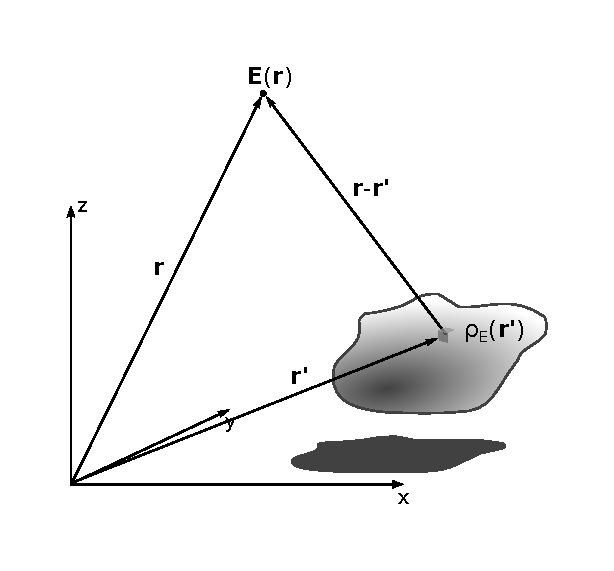
\includegraphics[width=0.5\textwidth]{../Figures/electricFieldcoord.pdf}
   \caption{
      The electric field $\boldsymbol E (\boldsymbol r)$ (at position $\boldsymbol r$)
      due to the charge distribution $\rho_E$ located at $\boldsymbol{r'}$.
   }
   \label{fig:electricField}
\end{figure}
%
However, it is usually simpler to calculate the electric potential $\Psi$
\begin{align}
   \label{electricPotential}
   \Psi(\boldsymbol{r}) 
   &= \frac{1}{4 \pi \varepsilon_0} \int \frac{1}{\big|\boldsymbol{r} - \boldsymbol{r'}\big|} 
                                                           \rho(\boldsymbol{r'}) d\!\boldsymbol{r'}
\end{align}
first and then calculate the electric field from
\begin{align}
   \boldsymbol{E} = - \nabla \Psi.
\end{align}
This might in some situations, where do do not necessarily know $\rho$ but only the total amount of 
charge, also be to tough to handle analytically. In situations like these it is better to use
Poisson's equation
\begin{align}
   \label{poisson}
   \nabla^2 \Psi= - \frac{1}{\varepsilon_o} \rho,
\end{align}
which together with appropriate boundary conditions, is equivalent to Eq.\eqref{electricPotential}.
Very often, we are interested in finding the potential containing no charge (because the charge is 
located on the outside of our region of interest. In such cases Eq. \eqref{poisson} reduces to
Laplace's equation (\cite{Griffiths}, p.110-111)
\begin{align}
   \label{laplace}
   \nabla^2 \Psi = 0.
\end{align}
According to the \textit{Uniqueness Theorems}, the solution to Laplace's equation is uniquely 
determined in some volume if the potential is specified on the boundary of the volume. This
easily extends to Poisson's equation by further requiring, in addition to the 
potential on the boundary, that the charge distribution throughout the region is known.
\\
\\
When considering conductors, charge are allowed to move freely and  might start to rearrange themselves,
leading to the \textit{Second uniqueness theorem}, which states that the potential in a given volume,
surrounded by conductors is uniquely determined if the total charge on each conductor is given.
\\
\\
The uniqueness theorem grants an enlarged mathematical freedom in the approach of finding the potential
of a region of space. This is because the boundary uniquely determines the potential in the region enclosed
region and any approach giving the correct boundary conditions would give you the correct potential 
function through Laplace's equation Eq. \eqref{laplace}. This allows the use of tricks, like for example
the classical \textit{method of images} (\cite{Griffiths}, p.116-121).





\subsection{Polarizability}
When a neutral atom is placed in an electric field $\boldsymbol{E}$, the field tries to rip the
atom apart by pushing the nucleus in the direction of the field and the electrons in the opposite direction.
Because of the attraction between the positive and negative charge within the atom, an equilibrium displacement
of the electrons compared to the nucleus is achieved, leaving the atom polarized and giving it a
dipole moment. The dipole moment can be approximated by
\begin{align}
   \boldsymbol{p} = \alpha \boldsymbol{E},
\end{align}
where $\alpha$ is the atomic polarizability and may depend on the detailed structure of the atom.
For more complicated situations, like an asymmetrical molecule, the gained dipole moment of the 
molecule does not necessarily have to be in the same direction as the applied electric field.
In such a case, the scalar polarizability in the expression above is replaced by a polarizability tensor
\begin{align}
   \boldsymbol{\alpha} = 
\begin{bmatrix}
   \alpha_{xx}   &   \alpha_{xy}  &  \alpha_{xz}  \\
   \alpha_{yx}   &   \alpha_{yy}  &  \alpha_{yz}  \\
   \alpha_{zx}   &   \alpha_{zy}  &  \alpha_{zz} 
\end{bmatrix}
.
\end{align}
In this way, an applied eletric field induces many dipole moments in a material. In addition,
any polar molecules will be subject to a torque, aligning it to the direction of the field.
These two mechanisms leads to the polarization $\boldsymbol{P}$ of the material
\begin{align}
   \boldsymbol{P} = \text{dipole moment per unit volume} = \varepsilon_0 \chi_e \boldsymbol{E}.
\end{align}
In the above expression, there has been assumed a linear dielectric media, where $\chi_e$ is the electric 
susceptibility and depends on the microscopic structure of the material, in addition to the external 
temperature (\cite{Griffiths},p.160-166, 179)



\subsection{Plasmons}

\subsection{\textbf{The Drude model} \cite{Hofmann} }
Defining the differences between the electrical properties of metals, semiconductors and insulators
is not a trivial matter. To put it simple, metals are good conductors, while semiconductors and 
insulators are not. However, semiconductors such as silicon conduct electrisity relatively well,
so the picture is not quite that simple.
\\
\\
A simple model, with fundamental importance regarding electrical conductivity, was suggested by
P. Drude in an attempt to explain the observed properties of metals. It is assumed that the 
electrons in a solid behave like a classical gas and do not interact with each other whatsoever.
Coloumb interaction is also neglected. This is known as the \textit{independent electron approximation}. 
The electron gas can be viewed as negatively charged particles bouncing about
immobile immobile positively charged ion cores. The only form of interaction in this model
are instantaneous collision between the electrons and ions; see Figure \ref{fig:DrudeModel}. 
The simplification of removing the Coloumb ion-electron interaction is called the 
\textit{free electron approximation}
%
\begin{figure}[h!]
  \centering
   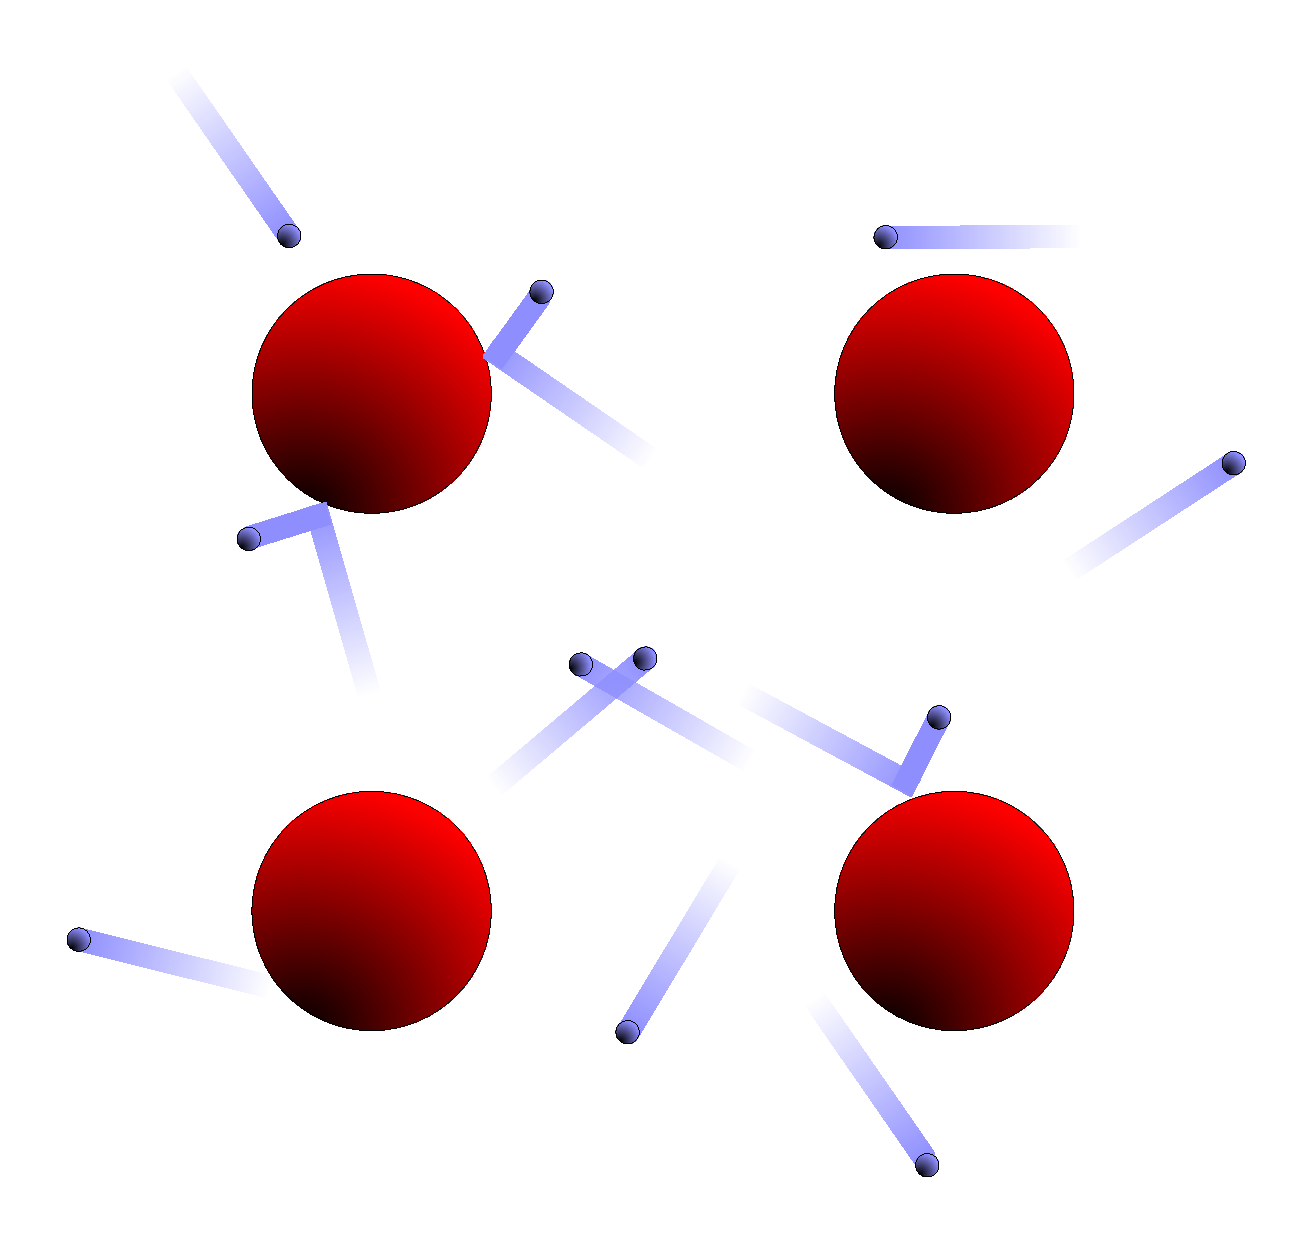
\includegraphics[width=0.5\textwidth]{../Figures/DrudeModel.pdf}
   \caption{ 
      The Drude model. A non-interacting electron gas (blue) is swirling around and colliding with 
      stationary positive ion cores (red). 
      Since all Coloumb forces are neglected together with electron-electron
      collsion, this ion-electron interaction is the only one being considered.
   }
   \label{fig:DrudeModel}
\end{figure}
%
The electrons reach thermal equilibrium with the lattice through the collisions, giving them
the kinetic energy:
\begin{align}
   \frac{1}{2}m_e v_t = \frac{3}{2}k_B T.
\end{align}
The average time between two collisions is called the relaxation time $\tau$, with the 
corresponding mean free path defined as $\lambda  = \tau v_t$. The probability for a 
electron to collide per unit time is assumed to be $1/\tau$. 
\\
\\
It is necessary to determine the conduction electron density $\rho_{c,e}$ in order to describe
properties such as electrical conductance. Assuming that every atom contributes 
every electron in its outermost shell $N_e$, e.g. that alkali metals contribute $N_e = 1$ and 
that earch alkaline earth metals contribute $N_e = 2$ etc. The number of atoms $N_a = \rho_m /m_a$, 
where $\rho_m$ is the density of the metal in [kg/m$^{-3}$] and $m_a$ is the atomic mass in [kg] 
(mass per atom).

\subsection{Conductivity; the Drude model}
Subjecting the drude metal of an electric field $\boldsymbol E$ will lead to a drift of the electrons
\begin{align}
   \frac{d \boldsymbol v}{dt} m_e = -e \boldsymbol E ,
\end{align}
where $e$ is the elementary charge. The solution is given by
\begin{align}
   \boldsymbol v (t) = \frac{-e \boldsymbol E t}{m_e}.
\end{align}
Assuming that the drift montion is destroyed in a collision, the average drift speed 
of the electrons become
\begin{align}
   \bar{\boldsymbol v }(t) = \frac{-e \boldsymbol E \tau}{m_e},
\end{align}
which is very slow compared to the thermal movement of the electrons $v_t$.
\\
\\
Considering an area $A$ perpendicular to the electric field, the amount of charge passing through 
the area is $-e n_e | \bar{\boldsymbol v} | A $ and the resulting current density would be
\begin{align}
   \boldsymbol j = n  \bar{\boldsymbol v} (-e) = \frac{n_e e^2 \tau}{m_e} \boldsymbol E \equiv \sigma \boldsymbol E = \boldsymbol E / \rho.
\end{align}
This is the familiar Ohm's law, with the conductivity 
\begin{align}
\sigma = \frac{n_e e^2 \tau}{m_e}
\end{align}
and the resistivity $\rho$. The $e^2$ dependence comes from the size of the pulling force
due to the electric field, i.e. how fast the particles move, and the other is how the same
charge, now moving, defines the current. This also means that we would get the same 
result for carriers with charge $e$ instead of $-e$, which would be the case for semiconductors
with positive holes.

\subsection{Optical reflectivity of drude metals}
The optical properties of materials are described by the complex refractive index $N(\omega)$ or 
the dielectric constant $\varepsilon(\omega)$. 
To explain the reflectivity of metals we can concider an electron in an electromagnetic 
field induced by an optical incident wave with wavenumber $q = 2\pi N/\lambda_0$, where 
$\lambda_0$ is the wavelength of the wave in free space.\\
If $\omega$ is low, we basically retain the DC behavior. However, if $\omega$ is so high that 
$1/\omega \ll \tau$, the electrons does not manage to react fast enough and the collisions with 
the ions altogether can be ignored (this is fulfilled for optical frequencies when $\tau=10^{-14}$s). 
The electrons can now be treated as completely free, and a single electron follows
\begin{align}
   m_e \frac{d^2x(t)}{dt^2} = -e E(t) = -e E e^{-i \omega t}.
   \label{freeElectronGas}
\end{align}
A good ansatz for the solution is setting $x(t) = xe^{-i \omega t}$, which mean that 
the electron is oscillating along with the electric field. This gives an amplitude of
\begin{align}
   x = \frac{eR}{m_e \omega^2}.
\end{align}
The corresponding polarization due to the dipole moment of $-ex$ for a solid with conduction electron
density $n_e$ is
\begin{align}
   P = -n_e ex = -\frac{n_e e^2E}{m_e \omega^2}.
\end{align}
From the constitutive relation
\begin{align}
   D = \varepsilon \varepsilon_0 E = \varepsilon_0 E + P,
\end{align}
we get that 
\begin{align}
   \varepsilon = 1 + \frac{P}{\varepsilon_0 E} = 1 - \frac{n_e e^2}{\varepsilon m_e \omega^2}
   \equiv 1 - frac{\omega_p^2}{\omega^2},
\end{align}
with the plasma frequency $\omega_p$ defined as
\begin{align}
   \omega_p = \frac{n_e e^2}{m_e\varepsilon_0}.
\end{align}
We can distinguish between two different cases and resulting outcome can
be seen from the the electromagnetic plane wave
\begin{align}
   \boldsymbol E (z,t) = \boldsymbol E_0 e^{i(2\pi N z/ \lambda_0 - \omega t)}.
\end{align}
In case 1) $\omega < \omega_p$ 
and $\varepsilon$ is a real and negative, $\varepsilon = \Re\{\varepsilon\} < 0$.
Therefore, $N = \sqrt{\varepsilon}$ is purely imaginary, and the wave penetrating the solid
is exponentially damped. Because Eq.\eqref{freeElectronGas} contain no inelastic properties, nothing
is absorbed. The light that is not transmitted into the medium must therefore, due to energy conservation, be
reflected back. 
For $\omega > \omega_p$, the dielectric constant is real and positive ,$\varepsilon = \Re\{\varepsilon\} > 0$,
and so is, followingly, the index of refraction. The result is a plane wave that propagates 
into the metal. This explains why metals are so reflective, or shiny. They are reflective for 
low-frequency light, but transparent for high-frequency light. The transition happens
at the plasma frequeny, which can be calculated solely from the conduction electron density of 
the metal. For most metals, the plasma frequency is in the far UV region, making them reflective 
in the visible range. Frequently, the plasma energy $\hbar \omega_p$ is used instead of the plasma frequency
$\omega_p$.

\subsection{Shortcomings of the Drude model}
The quenstionable assumptions of the Drude model is the removal of the electron-electron interaction
together with all the Coloumb forces. In addition, the assumption of treating the electrons as 
particles is not justified due to the fact that their de Broglie wavelength, in the case of thermal
electrons, is in the order of nanometers. The assumption would however only satisfy electrons moving
in structures much larger than the de Broglie wavelength.
\\
\\
The resulting conductivity of the model is not high enough at low temperatures, and is due to the
assumption of a fixed mean free path, given by the atomic spacing. Apparantly, at low temperature,
the electrons manage to sneak past the other electrons and ions. 
\\
\\
Also, the conductivity of alloys, in which impurities drastically reduce the conductivity, finds no
justification in the Drude model. 


\subsection{\textbf{Dielectrics}}
\subsection{Microscopic polarization}
There are several mechanismc causing microscopic electric dipole moments that lead to macroscopic 
polarization. E.g. displacement of electronic clouds and core, opposite displacement of the ions 
in a solid or
orientation of permanent dipoles such as water molecules, called orientational polarization.

\subsection{The local field}
To calculate the microscopic polarizability $\alpha$ of the atoms making up the solid, start with
the constitutive relation and assume that $\boldsymbol P$ can be written as the total dipole moment 
per unit volume
\begin{align}
   \boldsymbol P = (\varepsilon - 1 ) \varepsilon_0 \boldsymbol E = \frac{N}{V} \boldsymbol p = \frac{N}{V}\alpha \boldsymbol E.
   \label{nonLocalP}
\end{align}
Because a microscopic dipole within the solid does not simply feel the average electric field 
$\boldsymbol E$ but a microscopic local and stronger electric field $\boldsymbol E_{loc}$, the polarizability
can bot be correctly calculated from the above expression.
Without derivation, the approximate local field can be given by
\begin{align}
   \boldsymbol E_{loc} = \frac{1}{3}(\varepsilon + 2) \boldsymbol E.
\end{align}
So, with
\begin{align}
   \boldsymbol P = \frac{N}{V}\alpha \boldsymbol E_{loc}
\end{align}
and approximating the polarization $\boldsymbol P$ with Eq.\eqref{nonLocalP}, 
we get the so-called Clausius-Mossotti relation
\begin{align}
   \alpha = \frac{\varepsilon - 1}{\varepsilon + 2} \frac{3 \varepsilon_0 V}{N},
\end{align}
relating the atomic polarizabiliy to the dielectric constant.

\subsection{Frequency dependence of the dielectric constant}
The frequency dependent permittivity  $\varepsilon (\omega)$ is usually called the dielectric function.
For insulators, $\varepsilon(\omega)$ is complex and energy can be resonantly transferred to the solid
for certain frequencies. $\varepsilon(\omega)$ implies a frequency dependence of the refractive
index $N(\omega)$. Most of the frequency dependence can be explained by a simple idea 
combined with knowledge about the polarization mechanisms and how the different polarization mechanisms
manages to keep up with the oscillating electric field. E.g. orientation polarization and ionic polarization
does not manage to oscillate fast enough at higher frequencies, while the atomic polarization will, see
Figure \ref{fig:polarizationContribution}.
%
\begin{figure}[h!]
  \centering
   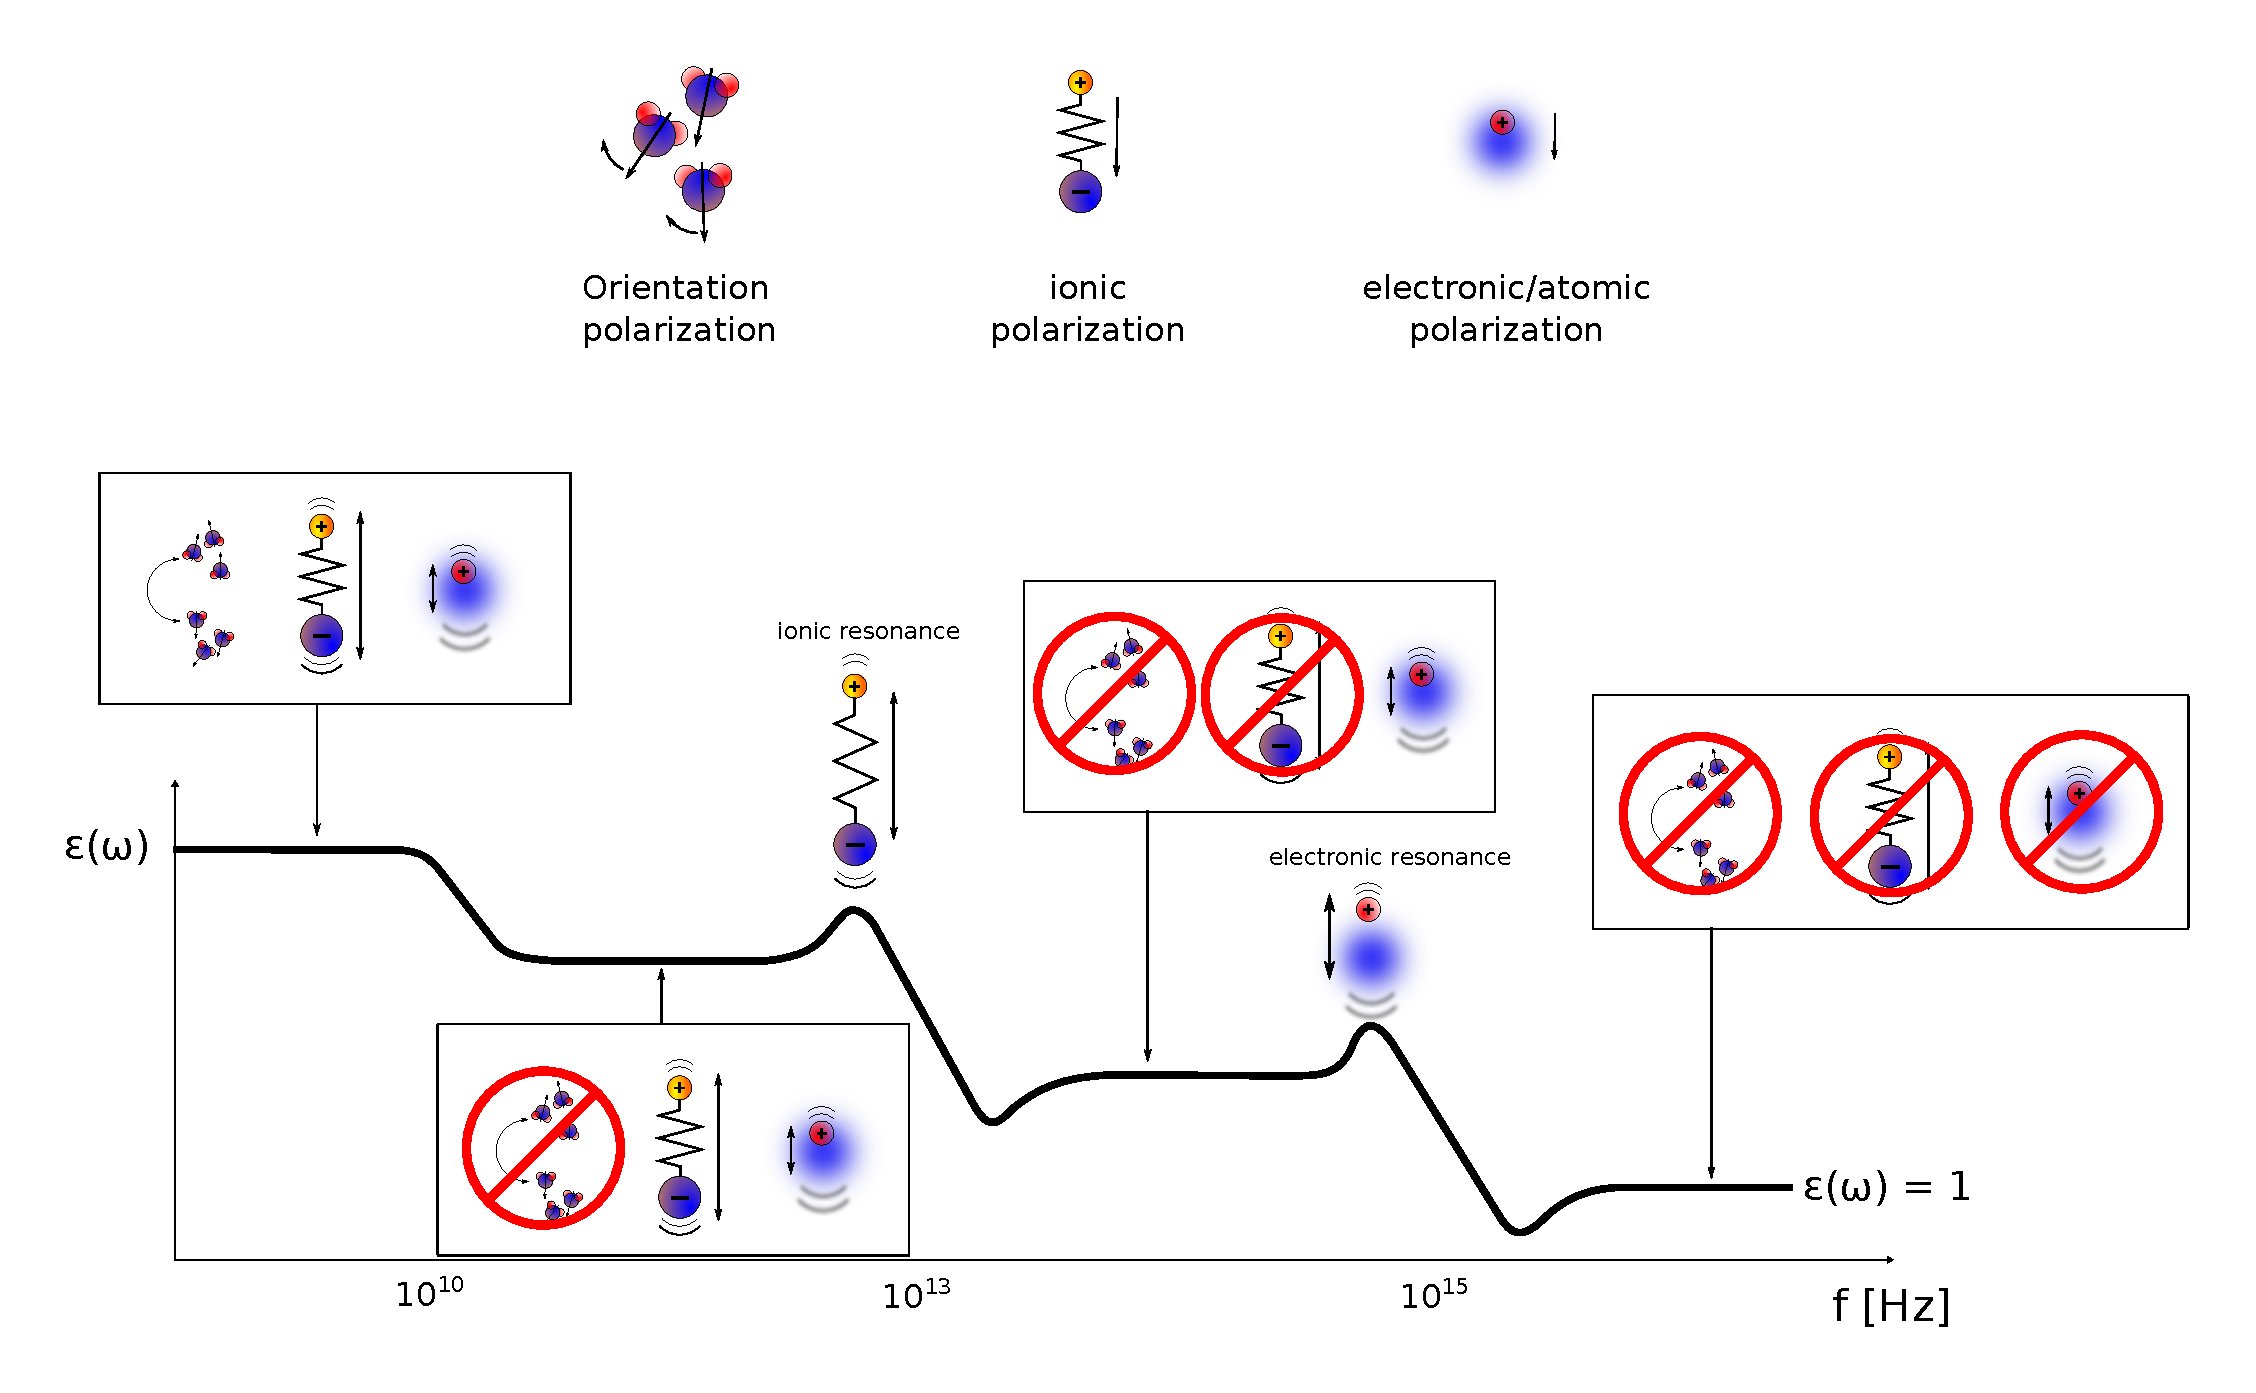
\includegraphics[width=1.0\textwidth]{../Figures/polarizationContributionToPermittivity.pdf}
   \caption{ 
      The contribution of orientation, ionic and electronic polarization. As the frequency
      of the applied electric field increases, the different polarization mechanisms fail to remain in 
      step with the field when above a characteristic frequency. At sufficiently high 
      frequencies the material no longer manages to polarize and the dielectric constant drops 
      to 1, corresponding to the permittivity of free space. Figure is adapted from 
      \cite{cambdridgePermittivityPage}.
   }
   \label{fig:polarizationContribution}
\end{figure}
%
\\
\\
For a quntitative description of the frequencydependence of $\varepsilon$ we can consider a simplified
version of ionic vibration.
Light can couple to optical phonons, e.g in ionic crystals where the phonons correspond to
an out-of-phase virbation of the positive and negative ions in the unit cell. 
These vibrations can be approximated by independent harmonic oscillators driven by an electric field
$E ^{-i\omega t}$, with one such oscillator per unit cell of the crystal. Each oscillator have a 
resonant frequency of $\omega_o = (2\gamma/M)^{1/2}$, where $\gamma$ is the force constant and
$M$ is the reduced mass of the two ions. The motion is damped by a term proportional to the velocity
$\eta d\!x\!/\!d\!t$ and represents the excitation of other vibrations in the material,
due to the large displacement. 
The resulting equation of motion is that of a driven harmonic oscillator with damping
\begin{align}
   \frac{d^2x}{dt^2} + \eta \frac{dx}{dt} + \omega_0^2 x = \frac{eE}{M}e^{-i\omega t}.
\end{align}
A good ansatz for the solution is 
\begin{align}
   x(t) = Ae^{-i \omega t},
\end{align}
resulting in the amplitude
\begin{align}
   A &= \frac{eE}{M} \frac{1}{\omega_0^2 - \omega^2 - i \eta \omega}  \\
     &=  \frac{eE}{M} \Bigg[ \frac{\omega_0^2 - \omega^2}{(\omega_0^2 - \omega^2)^2 +\eta^2 \omega^2} 
+ \frac{i\eta \omega}{(\omega_0^2 - \omega^2)^2 + \eta^2 \omega^2} \Bigg]
\end{align}
Using this as the ionic vibration, we can calculate the total polarization for a crystal with
$N$ unit cells and volume V. Considering only one type of ions with a density $N/V$ and effective
atomic polarizability $\alpha$, assuming both ionic and atomic polarization, $P_i(\omega)$, $P_a(\omega)$,
the result reads
\begin{align}
   P(\omega) = P_i(\omega) + P_a(\omega) = \frac{N}{V}eA(\omega)e^{-i \omega t} + \frac{N}{V}\alpha E e^{-i \omega t}.
\end{align}
When dealing with two types of ions like in a NaCl crystal, the different polarizabilities can be
taken care of by a suitable definition of $\alpha$. The resulting dielectric function can be calculated
from
\begin{align}
   \varepsilon_0 \varepsilon (\omega) E(\omega) = P(\omega) + \varepsilon_0 E(\omega),
\end{align}
giving
\begin{align}
   \varepsilon (\omega) &= \frac{P(\omega)}{\varepsilon_0 E e^{-i \omega t}} + 1  \\
                        &= \frac{NeA(\omega)}{V\varepsilon_0} + \frac{N \alpha}{V \varepsilon_0} + 1 \\
                        &= \frac{NeA(\omega)}{V\varepsilon_0} + \varepsilon\!_{_{opt}}.
\end{align}
Here, $\varepsilon_{opt}$ is the high frequency or optical limit, where the fields move to quickly for the 
ions to respond and $P_i(\omega) = 0$, i.e.
\begin{align}
   \varepsilon\!_{_{opt}} = \lim_{\omega\to\infty}\varepsilon (\omega)  
   = \frac{N \alpha}{V \varepsilon_0} + 1.
\end{align}
Plugging in the expression for $A(\omega)$ the real and complex values of the dielectric function 
$\varepsilon (\omega) = \varepsilon\!_{_{\Re\! e}} \!\! (\omega) + i \varepsilon\!_{_{\Im\! m}} \!\! (\omega)$ may be
written as
\begin{align}
   %\Re\! e [ \varepsilon (\omega) ]  &= \frac{Ne^2}{V\varepsilon_0 M} 
   &\varepsilon\!_{_{\Re\! e}} \!\! (\omega)  = \frac{Ne^2}{V\varepsilon_0 M} 
   \frac{\omega_0^2 - \omega^2}{(\omega_0^2-\omega^2)^2 + \eta^2 \omega^2} + \varepsilon\!_{_{opt}}
   \text{,}
   %
   %\Im \! m[ \varepsilon (\omega) ] &= \frac{Ne^2}{V\varepsilon_0 M} 
   &\varepsilon\!_{_{\Im \! m }} \!\! (\omega)  &= \frac{Ne^2}{V\varepsilon_0 M} 
   \frac{\eta \omega}{(\omega_0^2-\omega^2)^2 + \eta^2 \omega^2} 
\end{align}
The behaviour of the result is shown in Figure \ref{fig:dielectricResonance}
%
\begin{figure}[h!]
  \centering
   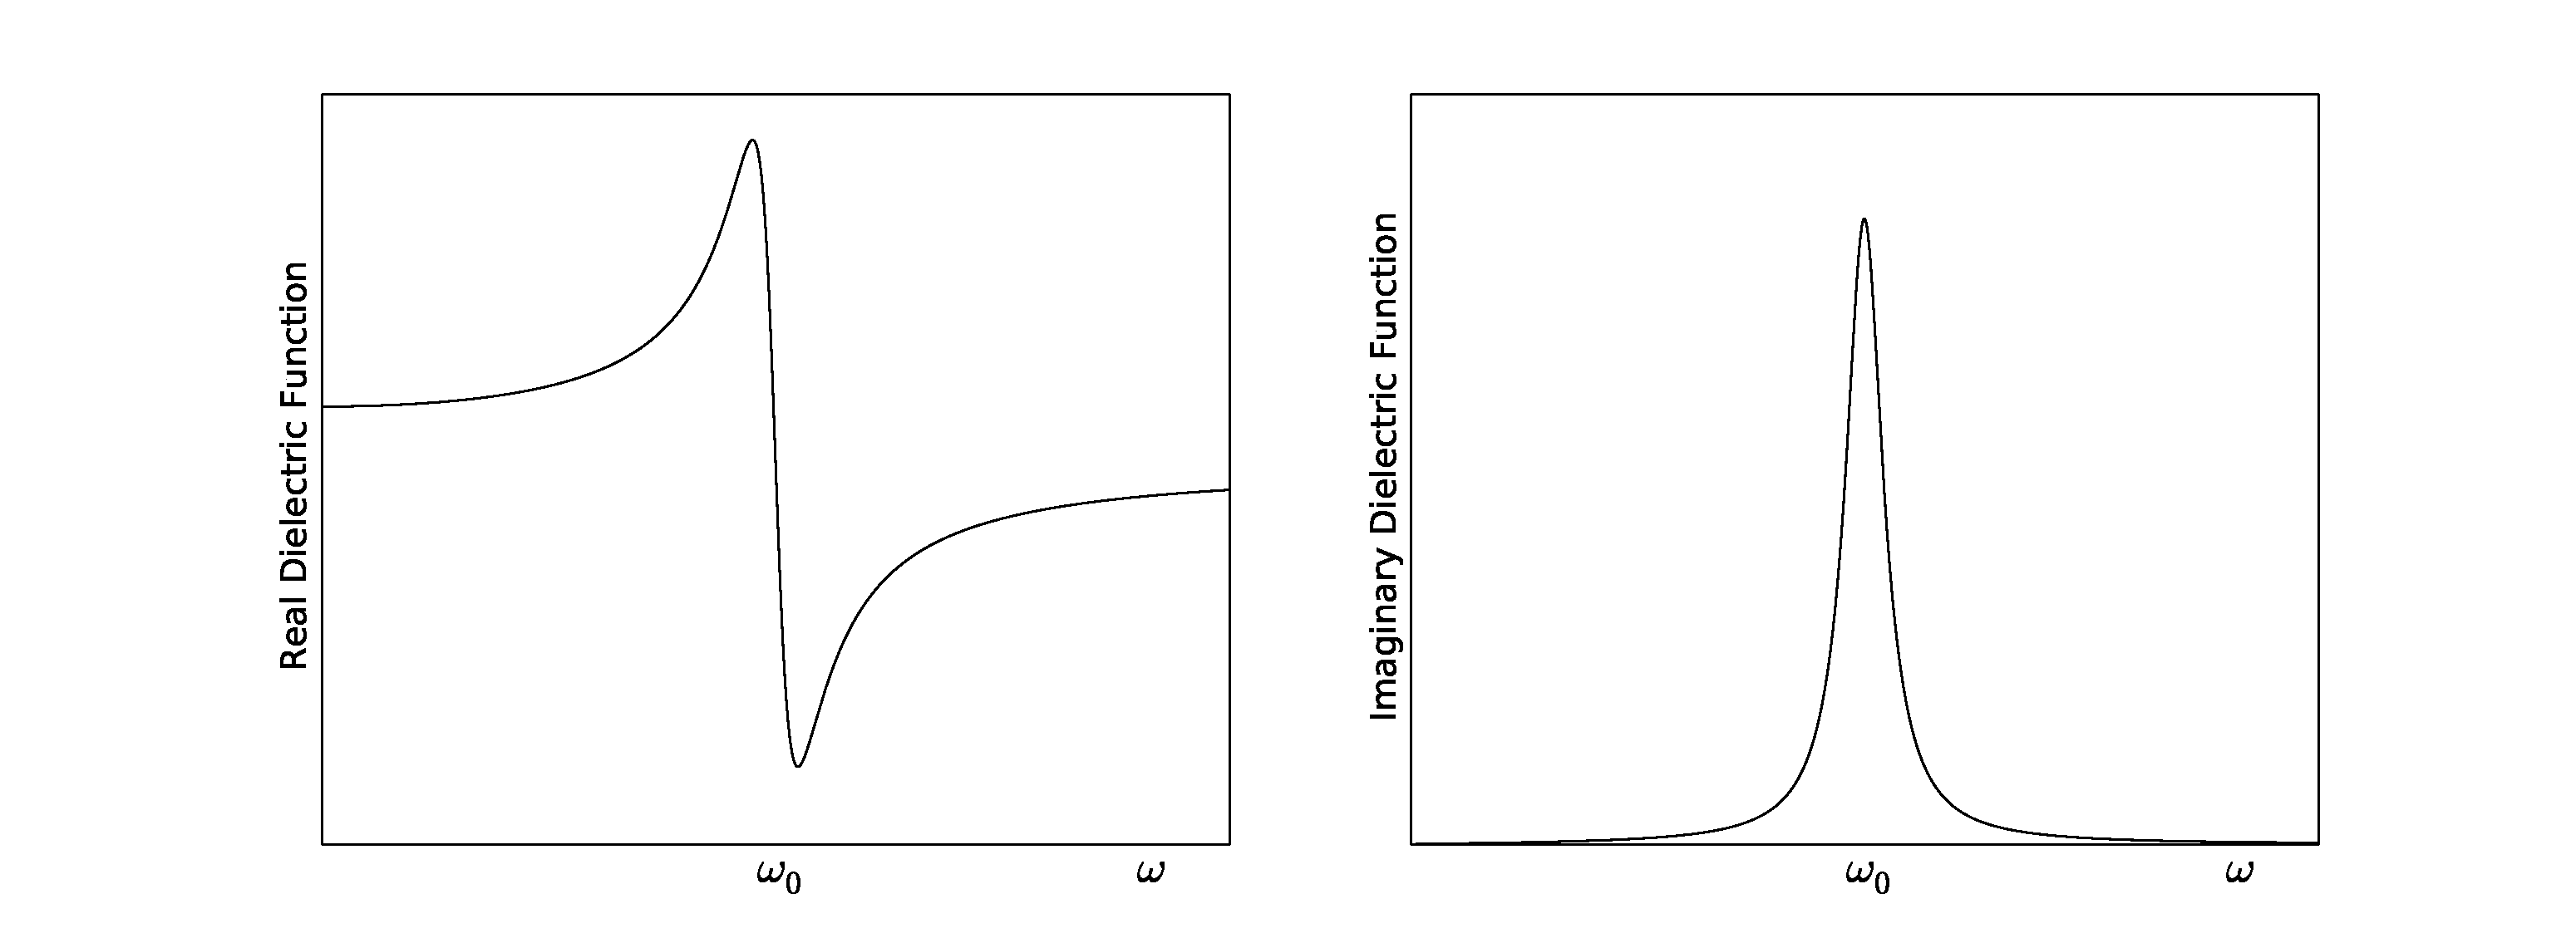
\includegraphics[width=1.0\textwidth]{../Figures/dielectricResonance.pdf}
   \caption{
      The dielectric function of a ionic crystal approximated by
      a driven harmonic oscillator with damping. The left and right figures show the behavior
      of the real and imaginary dielectric function close to
      the resonance frequency $\omega_0$.
   }
   \label{fig:dielectricResonance}
\end{figure}
%
The real part $\varepsilon\!_{_{\Re\! e}} \!\! (\omega)$ is almost constant away from the resonance
frequency, but its value is higher at lower frequencies due to the loss of the contribution from the
ionic polarization. The imaginary part $\varepsilon\!_{_{\Im\! m}} \!\! (\omega)$ is however zero 
everywhere except at the vicinity of the resonant frequency, where it shows a peak with a width
given by the damping coefficient $\eta$. 
\\
\\
To understand the meaning of $\varepsilon\!_{_{\Im\! m}} \!\! (\omega)$ and that the width
if its resonance peak is connected to the damping coefficient $\eta$, one can consider the
energy dissipation in the system. The instantaneous electrical power dissipated per unit 
volume is given by
\begin{align}
   P(t) = j(t)E(t) = j(t)Ee^{- i \omega t}
\end{align}
where j(t) is the curent density. In an insulator, there are no free currents, only polarization currents
\begin{align}
   j(t) = - \frac{\partial D}{\partial t} 
   = - \frac{\partial}{\partial t} \varepsilon \varepsilon_0 Ee^{- i \omega t}
   = i \omega \varepsilon \varepsilon_0 Ee^{- i \omega t}
\end{align}
The average dissipated power is found by averaging over one cycle $T = 2 \pi/\omega$
\begin{align}
   P = \frac{1}{T} \int_0^T E(t)j(t).
\end{align}
If $\varepsilon$ is purely imaginary, $j(t)$ is out of phase with $E(t)$ and their product will always
give a nonzero negative value,$-\varepsilon_0 \varepsilon\!_{_{\Im\! m}} \!\! (\omega) E^2$. On the other
hand, if $\varepsilon$ is purely real, the phase shift will be $\pi/2$ and the integral will give $P = 0$.
$\varepsilon\!_{_{\Im\! m}} \!\! (\omega)$ is therefore a measure of the energy dissipation of the
electric field due to the solid, and is obviously highest at the resonance.
\\
\\
The discussion explains some of the optical behaviour of the material. This is however not the
entire picture. E.g. the frequency dependence in the visible and UV region is not explained here.
These effects are due to the valence electrons, which would need a quantum mechanical description
of the electronic structure of the solid. From the band structure of solids, a qualitative
undestanding is obtainable. Figure \ref{fig:transitionResonance} shows regions of high photon absorbtion
due to the excitation of electrons, and how it is given by the imaginary dielectric function 
$\varepsilon\!_{_{\Im\! m}} \!\! (\omega) ? \varepsilon_i(\omega)$. Note that the photons do not have
enough energy to change the electrons wave vector
%
\begin{figure}[h!]
  \centering
   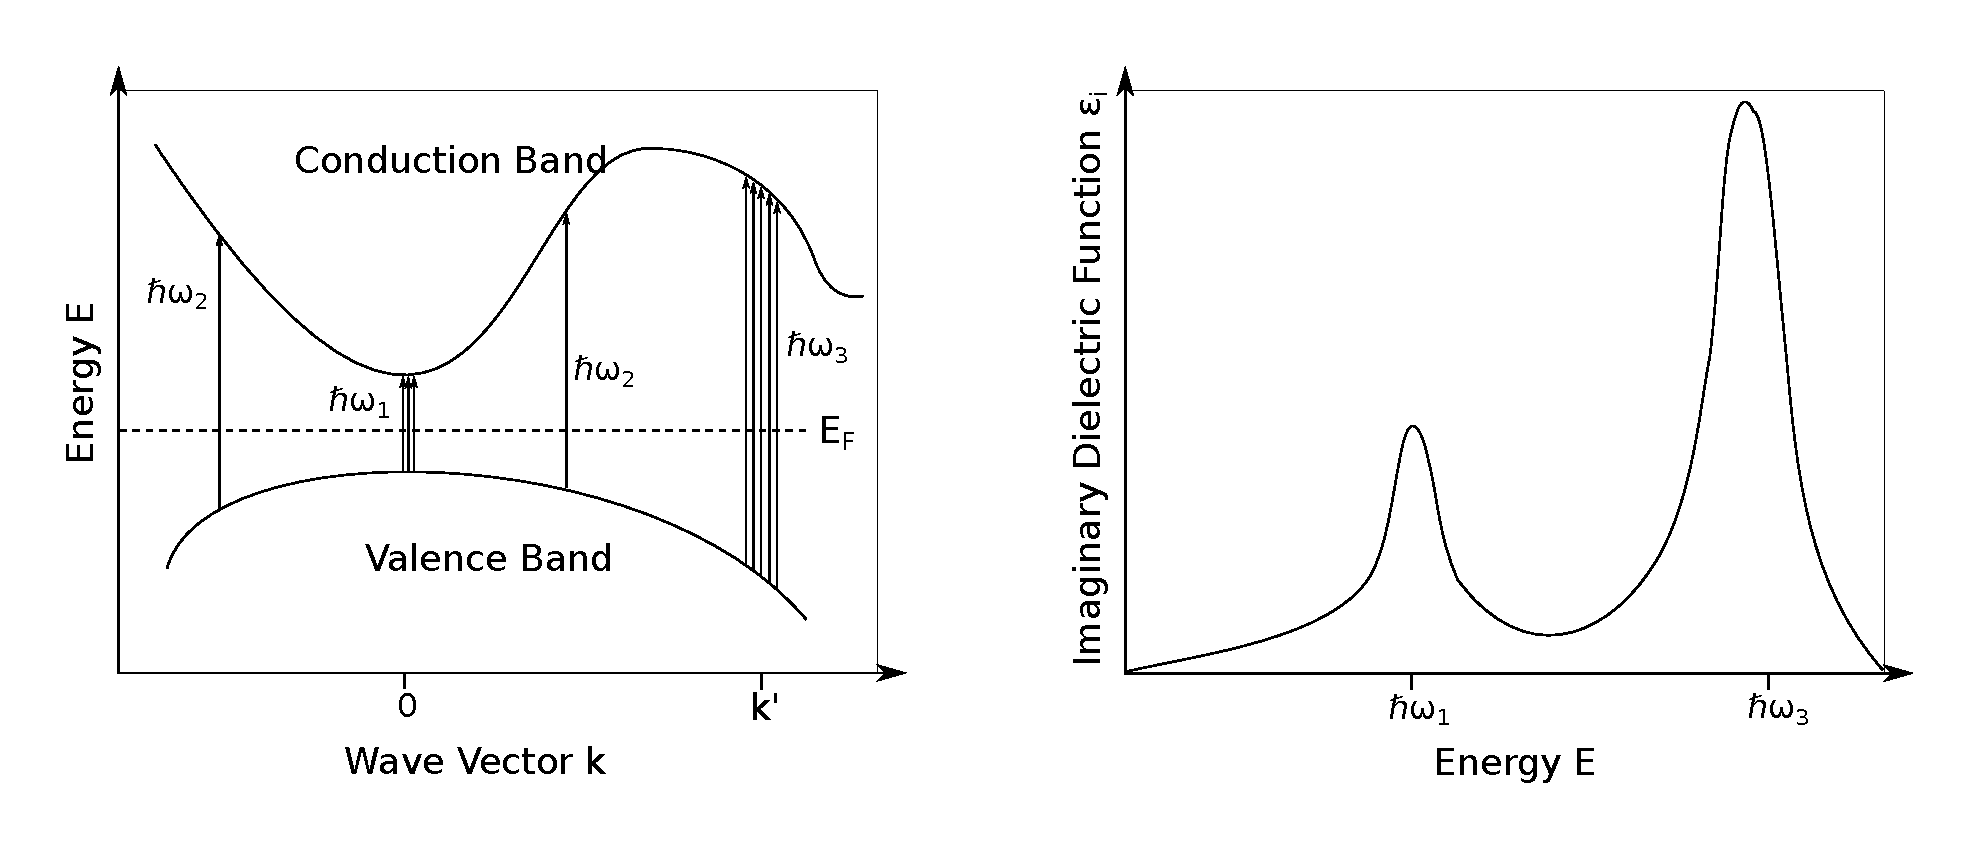
\includegraphics[width=1.0\textwidth]{../Figures/bandstructureVSdielectric.pdf}
   \caption{
      The left figure shows the photon-induced transitions between occupied and unoccupied states in the band 
      structure of a solid. $E_F$ is the fermi energy. 
      In the regions where the valence band and conduction bads are parallel,
      a certain photon energy can excite several states. Here, the parallel regions are located at
      $\boldsymbol k = 0$ and $\boldsymbol k = \boldsymbol k'$ and result in higher transitions density.
      These transitions correspond to absorbtion of the electromagnetic wave given by the imaginary part of
      the dielectric function $\varepsilon_i$. The resulting resonances in $\varepsilon_i$ due to 
      the absorbtion of the $\hbar \omega_1$ and $\hbar \omega_2$ transitions are depicted in the right
      figure.
   }
   \label{fig:transitionResonance}
\end{figure}
%






\begin{thebibliography}{9}

      \bibitem{Hofmann}
         Hofmann P.
         Solid State Physics, An Introduction.
         Wiley-VCH 2008; p.71-74,76-81

\end{thebibliography}




\subsection{Complex permittivity and index of refraction \cite[p.~169-170]{Jensen1985}}
%Jensen B: The Quantum Extension of the Drude-Zener Theory in Polar Semiconductors; p.169-188
The complex dielectric constant or relative permittivity 
$\widehat\varepsilon_r = \varepsilon_r + i \tilde\varepsilon_r$ of a material, is a measure of 
the material's response subject to an electromagnetic field. Here $\varepsilon_r$ and $\tilde\varepsilon_r$ 
denotes the real and imaginary components, respectively.
The relative permittivity is related to
the square of the refractive index, 
\begin{align}
   N^2 = \widehat\varepsilon_r
   \label{compEps}
\end{align}
which determines the optical properties of a given material.
It is like the dielectric constant complex
\begin{align}
   N = n + i k.
\end{align}
The real and imaginary refractive indicies are denotes by $n$ and $k$, respectively
The choice of sign convention, i.e. using $n+ik$ rather than $n-ik$, is determiend by 
the choice of the sign in the in the plane wave solution,
$\exp i(\boldsymbol q \cdot \boldsymbol r - \omega t )$, of
Maxwell's equations.
%The refractive index is also related to the conductivity $\sigma$
%\begin{align}
   %2nk = \frac{4\pi \sigma}{\omega}.
%\end{align}
%
From Eq.\eqref{compEps}
\begin{align}
   \widehat{\varepsilon}_r &= N^2 \\
   \varepsilon_r + i\tilde{\varepsilon}_r &= (n + ik)^2 \\
   \varepsilon_r + i\tilde{\varepsilon}_r &= n^2 - k^2 + i2nk,
\end{align}
and with some simple comparison, the components of the permittivity can be expressed as
\begin{align}
   \varepsilon_r &= n^2 - k^2     &\tilde{\varepsilon}_r  &= 2nk.
\end{align}
Taking the absolute value or modulus,
\begin{align}
   &\big|\widehat\varepsilon_r\big|   = \sqrt{ \varepsilon_r^2 + \tilde{\varepsilon}_r^2} \\
   &\big|\widehat\varepsilon_r\big|   = \sqrt{ (n^2 - k^2)^2 + (2nk)^2} \\
   &\big|\widehat\varepsilon_r\big|^2 = n^4 + 2n^2k^2 + k^4 \\
   &\big|\widehat\varepsilon_r\big|^2 = (n^2 + k^2)^2 \\
   &\big|\widehat\varepsilon_r\big|   = n^2 + k^2,
\end{align}
and putting it all together, gives the real and imaginary parts of $N$ expressed through the 
relative permettivity
\begin{align}
   n      &= \Bigg( \frac{\big|\widehat\varepsilon_r\big| + \varepsilon_r}{2}           \Bigg)^{\frac{1}{2}} 
           %= \Bigg( \frac{\big|\widehat\varepsilon  \big| + \varepsilon}{2\varepsilon_0}\Bigg)^{\frac{1}{2}}
  &k &=      \Bigg( \frac{\big|\widehat\varepsilon_r\big| - \varepsilon_r}{2}           \Bigg)^{\frac{1}{2}} 
           %= \Bigg( \frac{\big|\widehat\varepsilon  \big| - \varepsilon}{2\varepsilon_0}\Bigg)^{\frac{1}{2}}
\end{align}

Considering a plane wave with a complex wave vector $\widehat q = q + i \tilde q$ moving in the material
\cite[p.~402]{Griffiths}
\begin{align}
  e^{i(\widehat q z - \omega t )} 
  = e^{-\tilde q z} e^{i q z - \omega t )} ,
\end{align}
one sees that the wave is attenuated. 
The quantity $\alpha \equiv 2 \tilde q$ is called the absorption coeffiecient
and is proportional to the optical conductivity $\sigma$, to $\tilde\varepsilon$, and to $k$:
\begin{align}
   n\alpha = &\frac{4 \pi \sigma}{c} = \frac{\omega}{c} \tilde\varepsilon\\
                     &\Downarrow \\
   \frac{\alpha}{2} = &\frac{\omega}{c}k = \frac{1}{\delta}
\end{align}
$k$ is usually called the extinction coefficient and is essentially the ratio of the
free-space wave frequency $\omega$ to the skin depth $\delta$.\\


%Experimentally, $n$ and $k$ are found from measurements of the reflectivity R of a bulk, opaque sample
%and the transmittance T of a slab, which are given in terms of $n$ and $k$ as
$n$ and $k$ can be found experimentally by measuring the reflectivity R of a bulk, opaque sample,
in addition to the transmittance T of a slab, which are given in terms of $n$ and $k$ as
\begin{align}
   R &= \frac{(n-1)^2 + k^2}{(n+1)^2 + k^2} \\
   T &= \frac{ (1-R)^2 e^{-2\omega k d / c} }{ 1-R^2 e^{-4\omega k d / c} },
\end{align}
where $d$ is the sample thickness. The slab multiple-reflection effects are averaged,
so that interface fringes are not resolved.
%
\begin{thebibliography}{9}

      %Main article for dielectric function vs refractive index:
      \bibitem{Jensen1985}
       Jensen B.
       The quantum extension of the Drude-Zener theory in polar Semiconductors.
       Handbook of optical constants of Solids, Five-Volume 1997 (1985??)(9)<-it's chapter 9;169-170

      \bibitem{cambdridgePermittivityPage}.
         Dissemination of IT for the promotion of Materials Science (2000)
         Variation of the dielectric constant in alternating fields.
         University of Cambridge 2004:
         http://www.doitpoms.ac.uk/tlplib/dielectrics/variation.php
         (24. August 2015).
         %My interp. of webpage source: 
         %Authors, title, stuff behind(like university?) year ,link (date of site access)
\end{thebibliography}


\newpage
\section{Plasmons}
Notes from Justin White 
http://large.stanford.edu/courses/2007/ap272/white1/

\textbf{Surface Plasmon Polaritons}
\begin{itemize}
\item
Surface Plasmon polaritons are collective longitudinal oscillations
of electrons near a material surface, strongly coupled to 
an electromagnetic wave.

\item 
Both bulk and surface plasmons have associated EM-waves, and can
consequently be described by Maxwell's equations. 

\item 
the coherent oscillations of electron motion can be encapsulated in
the dielectric constant of the material. 

\item
The basic form of the bulk and surface plasmon solutions are shown
below:
\begin{align}
E_{bulk} &= E_0 e^{k_x x - \omega t}\\
E_{spp} &= E_0e^{-\kappa |z|} e^{k_x x - \omega t}
\end{align}
The bulk plasmons are associated with purely transverse EM waves
($E\perp k$ and  $B \perp k$) and can only exist for 
$\omega < \omega_p$. 
For $\omega > \omega_p$: the wave-vector for bulk plasmons becomes
imaginary, giving an exponentially decaying wave, instead of a 
propagating wave. It is for this reason that most metals 
are highly reflective for visible light ($\omega <\omega_p$),
but transparent for ultraviolet light ($\omega > \omega_p$)

\item
Surface plasmons have an associated EM wave with both transverse 
and longitudinal field components. Such waves can only be excited
at the interface between a conductor and dielectric, and aretightly bound to the surface. The field reach their maximum at the interface 
($z=0$), and exponentially decay away from the surface.

\item 
The wave-vector of the surface plasmon mode $k_{spp}$ always lies
to the right of the free space wave-vector $k_0$ (in the dispersion 
diagram/relation), such that $\lambda_{spp} < \lambda_0$. this makes
 it impossible to directly launch a surface plasmon wave by
illumination with free-space radiation, because the free-space photons
simply do not have enough momentum to excite the surface plasmon.

As $\omega$ increases, $k_{spp}$ gets larger and larger, moving
further  away from $k_0$ (textit{??making it harder and harder 
for light to excite the surface plasmons??})d. As $k_{spp}$ increases,
the surface plasmon wave is more tightly bound to the surface.
This process has an upper limit of $\omega_{sp}$, the surface 
plasmon resonant frequency, which occurs when the dielectric 
constant of the metal and the dielectric have the same 
magnitude but opposite signs.

\item
\textbf{Excitation of Surface Plasmons}\\
High energy electrons that bombard a thin metalic film can
launch surface plasmons and a surface plasmons of a whole range
of wavelengths can be excited. However, only plasmons
far along the dispersion curve, where $k_{spp}$ is largest
are generally excited.
\\
\\
As mentioned previously, direct excitation of surface plasmons by 
free-space photons is not achievable because $k_{spp}$ is 
always greater than $k_0$; this can be seen from the dispersion
relation, where the surface plasmon dispersion relation always
lies to the right of the free space dispersion curve.\\
This can be overcome by back-side illumination through a material
with a higher index of refraction $n$, where the far field radiation
has a larger wave-vector ($k=nk_0$) 
(like done in a Kretschmann-Raether coupler) [5].
A surface plasmon will be efficiently excited when 
\begin{align}
k_{\parallel} = n k_0 \sin \theta = k_{spp}
\end{align}
A mor egeneral approach to launch surface plasmons with light
is the use of structured surfaces that are able to impart momentum
on the photon, enabling it to couple to the surface plasmon mode.
Anything from a single sub-wavelength disk or slit, to rectangular
or sinusoidal diffraction gratings are used for this type of coupling.
\textbf{A thorough overview of surface plasmon coupling 
and patterned and rough surfaces is given by Raether[6]}


\item Appendix: Derivation of Bulk and Surface Plasmons (see article).
\end{itemize}

Other Nice sources:
\begin{itemize}
\item Really nice article on Plasmons:\\
http://nanocomposix.com/pages/plasmonics

\item Article:\\
http://cdn.intechopen.com/pdfs-wm/44351.pdf

\item Surface Plasmon Theory(book?):\\
https://www.physik.hu-berlin.de/de/nano/lehre/Gastvorlesung%20Wien/Plasmonics%20Pitarke

\item Chemistry-blog:\\
http://www.chemistry-blog.com/2007/03/19/plasmonics-part-ii/

\item Mie theory: \\
http://www.orc.soton.ac.uk/publications/theses/1460T\_lnn/1460T\_lnn\_03.pdf
\end{itemize}




\newpage
\textbf{From Wikipedia}
\begin{itemize}
   \item \textbf{What are Plasmons?} \\
A plasmon is a quantum of plasma oscillation (quasiparticle from the quantization of plasma oscillations).
Plasmons are collective (a discrete number) oscillations of the free elctron gas density.
Plasmons can also couple with a photon to create another quasiparticle called a plasma polariton
(electromagnetic wave - electric/magnetic dipole-carrying exitation - coupling.
\\
\\
Plasmons can be described as oscillations of free elctron density with respect to
fixed positive ions in a metal. Imagine a cube of metal placed in an external 
electric field pointing to the right. Electrons will move the the left side and uncover
positive ions on the right side. The electrons will continue moving left until they
cancel the field inside the metal. Removing the field will make the electrons move back by their
mutual repulsion and attraction to the ions, leaving the electrons to oscillate back and forth,
at the \textbf{plasma frequency}, in a so called plasma oscillation.

\item \textbf{Plasma Oscillation, aka ''Langmuir waves''} \\
Rapid oscillations of electron density in conducting media such as plasmas or metals.
The oscillations can be described as an instability in the dielectric function of a free electron gas.
The frequency depends weakly on the wavelength of the oscillation.
\\
\\
'Cold' electrons (plasma oscillations)\\
If the thermal motion of the electrons is ignored and assuming infinite ion mass,
the charge density oscillates at the plasma frequency
\begin{align}
   \omega_{pe} &= \sqrt{\frac{n_e e^2}{m^* \varepsilon_0}}, \text{[rad/s] (SI-units)} \\
   \omega_{pe} &= \sqrt{\frac{4 \pi n_e e^2}{m^*}}, \text{(cgs-units)},
\end{align}
where $n_e$ is the number density of electrons, $e$ is the electric charge, $m^*$ is the effective mass of
the electron and $\varepsilon_0$ is the permittivity of free space. Since the frequency is independent of 
the wavelength, these oscillations have an infinite phase velocity and zero group velocity.
Note in addition that, if $m^*$ is the electron mass $m_e$, the plasma frequency $\omega_{pe}$
depends only on the physical constants and concentration of electrons $n_e$. The numeric expression is:
\begin{align}
f_{pe} = \frac{\omega_{pe}}{2 \pi} \approx 8980 \sqrt{n_e}, \text{[Hz]}
\end{align}
with $n_e$ in [cm$^{-3}$]
\\
\\
'Warm' electrons (plasma oscillations)\\
When the effects of the electron thermal speed $v_{e,th} = \sqrt{\frac{k_B T_e}{m_e}}$ are taken into account,
the electron pressure acts as an additional restoring force and the oscillations propagate with
frequency and wavenumber related by the longitudinal Langmuir wave:
\begin{align}
\omega ^2 = \omega_{pe} ^2 + \frac{3 k_B T_e}{m_e} k^2 = \omega_{pe} ^2 + 3k^2 v_{e,th}^2
\end{align}
called the 'Bohm-Gross dispersion relation'. If the spatial scale is large compared to
the Debye length (measure of a charge carrier's net electrostatic effect in solution, 
and how far those electrostatic effects persist), the oscillations are only weakly modified
by the pressure term, but at small scales the pressure term dominates and 
the waves become dispersionless with a speed of $\sqrt{3}v_{e,th}$. For such waves, however, the
electron thermal speed is comparable to the phase velocity, i.e.
\begin{align}
v \sim v_{p,th} \equiv \frac{\omega}{k},
\end{align}
so the plasma waves can accelerate electrons that are moving with speed nearly equal to the
phase velocity of the wave. This process often leads to a form of collisionless damping
called Landau damping. Consequently, the large-k portion in the dispersion relation is difficult to
observe and seldom of consequence.
\\
\\
In metal of semiconductor, the effect of the ions periodic potential must be taken into account. This is
usually done by using the electrons effective mass in place of $m$.

\item \textbf{Role of Plasmons} \\
Plasmons play a large role in the optical properties of metals. Light of frequencies below the
plasma frequency is reflected, because the electrons in the metal screen the electric field 
of the light. Light of frequencies above the plasma frequency is transmitted, because the
electrons cannot respond fast eneough to screen it. In mot metals, the plasma frequency is in the 
unltraviolet, making them shiny (reflective) in the visible range. 
In semiconductors, the valence electron plasma frquency is usually in the deep ultraviolet, which is why
they are reflective.
\\
The plasmon energy can often be estimated in the free electron model as
\begin{align}
   E = \hbar \sqrt{\frac{n_e e^2}{m^* \varepsilon_0}} = \hbar \omega_p
\end{align}




\item \textbf{Surface Plasmons (SPs)} \\
Surface plasmons (plasmons at the interface of two materials) interact strongly with light,
resulting in a polariton (usually occurs at metal or doped dielectric interface, 
which both have small Im($\varepsilon$) > 0 and big Re($\varepsilon$) < 0).
These surface electron oscillations can exist at the interface between
any two materials where the real part of the dielectric function changes sign across the interface
(e.g. a metal-dielectric interface like metal sheet in air).
\\
SPs have lower energy than \textbf{bulk (or volume)} plasmons, which quantise the longitudinal
electron oscillations about positive ion cores within the bulk of an electron gas (or plasma).
\\
\\
The charge motion in a surface plasmon always create electromagnetic fields outside (as well as inside)
the metal. The total excitation, including both the charge motion and associated electromagnetic field,
is called either a \textbf{surface plasmon polariton} at a planar interface, or a \textbf{localized
surface plasmon} for the closed surface of a small particle.
\\
\\
Surface Plasmon polaritons can be excited by electrons or photons. In the case of photons, it
cannot be done directly, but requires a prism, or a grating, or a defect on the metal surface.
\textit{??? Or like trunctated spheres on granular films???}.
\\
\\
At low frequency an SPP approaches the dispersionrelation in free space $\omega = ck$.
At high frequency, the dispersion relation reaches an asymptotic limit called the ''sufrace plasma frequency''.
\\
\\
As an SPP propagates along the surface, it loses energy to the metal
due to absorption and due to scattering into free-space or into other directions. The electric field
falls off evanescently perpendicular to the metal surface. At low frequencies, the SPP penetration depth into
the metal is commonly approximated using the 'skin depth formula'. In the dielectric, the field 
will fall off far more slowly. SPPs are very sensitive to slight perturbations within the skin depth and because of this, SPPs, are often sed to probe inhomogeneities of a surface
\\
\\
Surface plasmons have been used to control colors of materials and is possible since controlling 
the particle's shape and size determines the types of surface plasmons that can couple to it and 
propagate across it. This in turn controls the interaction of light with the surface.
These effects are illustrated by the historic \textit{stained glass} wich adorn medieval
cathedrals. In this case, the color is given by metal nanoparticles of a fixed size which interact
with the optical field to give the glass its vibrant color. To produce optical range surface plasmons
effects involves producing surfaces wich have features < 400nm.
\\
\\
Surface plasmons are very sensitive to the properties of the materials on which they propagate.


\item \textbf{Surface Plasmons Resonance (SPR)} \\
Surface plasmon resonance is the resonant oscillation of conduction electrons at the interface
between a negative and positive permittivity meterial stimulated by incident light. The resonance
condition is estalished when the frequency of incident photons matches the natural
frequency of surface electrons oscillating against the restoring force of positive nuclei.
\\
\\
Surface plasmon polaritons are surface electromegnetic waves that propagate in a direction parallel to
the metal/dielectric (or metal/valcuum) interface. Since the wave is on the boundary of the metal
and the external medium, these oscillations are very sensitive to any change of this boundary, such as
adsoption of molecules to the metal surface.
\\
\\
To describe the existence and properties of surface plasmon polaritons, one can choose from various models,
e.g. the \textbf{Drude Model}. The simplest way to approach the problem is to treat each
material as a homogeneous continuum, described by a frequency-dependent relative permittivity between 
the external medium and the surface (this is a complex dielectric function). In order
for the terms that describe the electronic surface plasmons to exist, the real part of the dielectric constant
of the metal must be negative and its magnitude must be greater than that of the dielectric.
This condition is met in the infrared-visible wavelength region for air/metal and water/metal interfaces (where
the real dielectric constant of a metal is negative and that of air or water is possitive).
\\
\\
Localized SPRs (LSPRs) are collective charge oscillations in metallic nanoparticles that
are excited by light. They exhibit enhanced near-field amplitude at the resonance wavelength.
This field is highly localiced at the nanoparticle and decays rapidly away from the nanoparticle/dielectric
interface into the dielectric background, though far-field scattering by the particle is also 
enhanced by the resonance. Light intensity enhancement is a very important aspect of LSPRs and
and localization means the LSPR has very high spatial resolution (subwavelength), lmited
only by the size of nanoparticles. Because of the enhanced field amplitude, effects that depend on the
amplitude such as magneto-optical effect are also enhanced by LSPRs.
\\
\\
In order to excite surface plasmoms in a resonant manner, one can use an electron or light beam
(visible and infrared are typical). The incoming beam has to match its momentum to that of the plasmon.\\
With p-polarization this is possible by assing the light through a block of glass to
increase the wavenumber (and the momentum) and achieve the resonance at a given wavelength and angle.\\
s-polarized light however cannot excite electronic surface plasmons.
\\
\\
When the surface plasmon wave interacts with a local particle or irregularity, such as a rough surface,
part of the energy can be re-emmited as light. This emitted light can be detected behind the metal film
from various diretions.


\item \textbf{The Drude Model}\\
Treats the behavior of electrons in a solid like a pinball machine. 
The electrons are small light balls in a sea of static, positively charged ions. The only 
form of action instantaneous collisions.


\item \textbf{Mie Scattering}\\
Mie theory is sometimes used for the collection of methods and solutions to Maxwell's equations
for scattering, by e.g. using geometries where one can write separate equations for the radial and angular
dependence of solutions. More broadly, ''Mie scattering'' suggests situations where the size of the
scattering particles is comparable to the wavelength of the light, rather than much smaller or much larger.
\end{itemize}

\begin{thebibliography}{9}

      \bibitem{} 

\end{thebibliography}


\newpage
\section{Article Notes}
\subsection{Thermochromism}
\cite{intelligentWindows} 
\textbf{Intelligent Themochromic Windows} \\
The use of air-conditioning systems to maintain comfortable working and 
living environments has become more common [1]. This leads to an increase in hte use
of electricity and a concurrent increase in carbon dioxide emmissions and other 
atmospheric pollutants formed in the electricity generation process. A self-propagating cucle results,
in which blobal warming due to increases in these greenhouse gases necessitates the increased 
use of air conditioning systems. Technology is thus required that can reduce the use of air conditioning
commercial and residential buildings to help break this cycle. \\
\\
(...) window coatings can reduce cooling costs or heating requirements [2]. 
Using thermochromic coatings as intelligent window coatings[1-7], which change
their optical properties with temperature; usually related to a structural pase change on passing through a 
critical temperature $T_c$. Thermochromic coatings would be applicable to climates where there are extreme 
changes in temperature over the year, for example, central and northern Europe, Japan, the United States, 
and Canada, which have hot summers and cold winters. \\
\\
Vanadium(IV) oxide; transition temperature $Tc = 68 ^{\circ}$C; visually and infrared trasnparent belov $T_c$ 
$\rightarrow$ solar radiation passes through, keeping the interior warm. Below $T_c$ it becomes infrared reflective
and preventing excessive heating, while remaining visually transparent.\\
\\
Critical temperature for vanadium is too high, but this can be lowered to $25^{\circ}$C uing dopants ([9]),
most efficiently with tungsten(loading of only 2 atom percent required), in thin films prepared by physical 
vapor deposition methods [10] and sol-gel spin or dip coating [11]. \\
\\
problem: low luminous transmittance of the glazing VO$_2$ film [10-13]. (could be solved with doping[4]
or anti-reflective coating ([12])). Also one needs a method where the thin films of the material
can be applied cheaply and efficiently to the glass ([17]).\\
\\
(p.394) Discussion of MST(metal-to-semiconductor transition) of VO$_2$ and structure 
changes through the MST. Discussion involves structure figures.\\
\\
Goodenough proposes antiferroelectric transition being the drivings force
for the MST in VO$_2$. $\rightarrow$ two transition temperatures: one due to antiferroelectric
distortion and one due to the crystallographic distortion. \\
\\
The next paragraph explains how doping of various elements varies the MST temperature. 
The most effective dopant in reducing the temperature is Tungsten (additional info about tungsten 
and after that it considers other dopants). \\
\\
Thinner thickness, stress and strain can also reduce the thermchromic transition temperature.\\
\\
A little bit on VO$_2$ thin film durability? \\
Methods of preparing Pure  and doped Vanadium(IV) Oxide Films:\\ 
Sol-Gel Method: forming thin films by dip- or spin-coating substrates with solutions of metal alkoxides. \\
PVD Method: energetically removing atoms/molecules under reduced pressure conditions, then to react with seed gas. \\ 
CVD method: chemical vapor deposition, in particular atmospheric pressure CVD (APCVD). \\
APCVD: deposit tin solid films from gaseous precursors onto a suitable substrate. (+Pictorial representation)\\
(and more on APCVD).\\
\\
Comparison of the above methods. \\
\\
3 atom percent tungsten(VI) $\rightarrow$ transition temperature reduced to $5^{\circ}$C.\\
1.9 percent $\rightarrow$ $29^{\circ}$C.\\
transition temperature decreases linearly with tungsten atom percent incorporation(Figure). \\
\\
Summary: intelligent TC glass with desired switch temperature($25-30^{circ}$C, obtainable using APCVD.
Mst of the problems regarding commercial use are solvable. Market in household, offices, factories and space
exploration.\\


\newpage
\cite{TCcommercialProducts} 
\textbf{Thermochromism in Commercial Products} \\
\begin{itemize}
\item Thermochromic liquid crystals: Periodicity between layers, PITCH, and constructive interference!. 
   TC liquid crystals can have a versatile range of colors and useful color changes bewteen -30 
   and 120$^{\circ}$C, often with very high temperature sensitivity. TC liquid crystals are only useful when
   they are in the liquid crystalline phase, which is a meso-phase (an intermediate phase of matter) between
   an isotropic liquid (high temperature) and crystalline solid (low temperature), which restricts the
   temperature range of theur applicability.
\item \textbf{Microencapsulation}: Defined as the coating of small solid particles, liquid droplets,
   or gas bubbles with a thin film or coating or shell material, and typical particle sizes are
   1 to 1000 $\mu$m ([20] Kirk-Othmer Encycloped. of chem. Tech. 4thEd). For three component organic mixtures,
   particle sizes are < 50 $\mu$m. \textbf{Micro encapsulation allows the additional advantage 
   of combinations of several narrow color ranges}, and very sharp color changes, 
      as well as protection of the coloring agent
   from the environment ([16] Nakasuji med flere. Chem.Abs.).
   \textbf{complex coacervation} and \textbf{interfacial polymerization} $\rightarrow$ processes to
   microencapsulate thermochromic materials! Also described! Nice to include if I use thin layer on my 
   granular film!
\item Smart window candidates: Fe$_3$O$_4$, FeSi$_4$, NbO$_2$, NiS, Ti$_2$O$_3$ and VO$_2$, which
   owe their temperature change to a semiconductor-to-metallic state transition 
   (aka \textbf{Mott transition temperature})
\end{itemize}



\newpage
\cite{TCqualitativeDescription} 
\textbf{A Qualitative Description of Thermochromism in Color Measurements} \\
\begin{itemize}
\item Wyszecki and Stiles stated ([2] color science), for TC transmitting filters, that the spectral
   transmittance curve at a given wavelength with a large positive slope usually dereases with increasing
   temperature. As a rule: steeper(positive) slope $\rightarrow$ greater temperature effect! \\
   The curve with negative slope is of minor importance, but often causes transmittance increase for
   increasing temperature (if it is important). \\
   \\
   Neutral samples (gray, white, black) did not exhibit TC, because their spectral reflectance curves
   have a small or no slope.
\item Assuming nonfluorescent, linear material which is "nice" with respect to polarization effects, then
   \begin{align*}
      1 = R_{\lambda} + A_{\lambda} + T_{\lambda}
   \end{align*}
   where, $R_{\lambda}$ is the reflectance, $A_{\lambda}$ is the absorbance and $T_{\lambda}$ is the
   transmittance of the sample.\\
   Considering \textbf{transmitting samples}, the intensity $I_{\lambda}$ transmitted through a 
   sample of thickness $d$ is given by
   \begin{align*}
      I_{\lambda} = I_{0 \lambda} e^{- \mu_{\lambda} d}
   \end{align*}
   where $\mu_{\lambda}$ is the absorption coefficient of the sample at wavelength $\lambda$.
   The optical density $D$ is then given by:
   \begin{align*}
      D = -\log(T_{\lambda}) = -\log(\frac{I_{\lambda}}{I_{0\lambda}}) = \mu_{\lambda} d \log e
      = \frac{\mu_{\lambda}}{\ln 10}
   \end{align*}
   For \textbf{opaque samples} there is no transmittance, but the optical density can be calculated
   from the reflected intensity $I_{R\lambda}$:
   \begin{align*}
      D_{\lambda} = -\log(\frac{I_{R\lambda}}{I_{0\lambda}}).
   \end{align*}
   The light reflected from the material is also exponentially attenuated, for opaque materials.
   Thus, $D=\frac{\mu_{\lambda}}{\ln 10}$ holds for reflected light if $d$ is the distance the
   reflected light has passed in the material.
\end{itemize}


\newpage
\cite{renewableSustainableEnergyRev}
\textbf{A Qualitative Description of Thermochromism in Color Measurements} \\
\begin{itemize}
\item
\end{itemize}

      
\newpage
\cite{Kamalisarvestani2013}
%\cite{coatingTechOfTCthinFilmSmartWindows}
\textbf{Performance, materials and coating technologies of thermochromic thin films on smart windows} \\
\begin{itemize}
\item A significant amount of energy is consumed to maintain thermal comfort in buildings, 
   a huge portion which is lost through windows. 
   smart windows obtained by thin films is the solution. The touchstone of performance 
   is the change in visible and infra-red transmission and reflectance!
\item A significant amount of the energy consumption in buildings are mainly due to HVAC (heating, ventilation 
   and air conditioning) devices, used to obtain thermal comfort,
   The building energy consumption in developed contries accounts for 20-40$\%$ of the total energy use.
   (including further details of US and China energy consumption). The building energy consumption is even more
   dominant in hot and humid regions, using one-third to half of the elextricity produced in some contries.
   Energy related carbon dioxide emmision. Motivates energy saving measures to reduce building energy losses and CO$_2$
   emissions.
\item Two approaches to increase energy efficieny (7-10)
   \begin{itemize}
      \item Active stratergies: improving HVAC systems and building lighting.
      \item Passive stratergies: improving the thermal properties of the building envelope (elementss
         separating the indoor from outdoor), i.e. thermal insulation to wall, cool coatings on roofs
                  and coated window glazings.
   \end{itemize}
\item Windows are known as one of the most energy inefficient components of buildings.(11) \\
      Improving the thermal performance of windows will result in reduced electricity costs 
      and less greenhouse gas emmissions. \\
      In addition to controlling transmitted IR radiation an ideal window should be capable 
      of sufficient transmission of visible light(12). \\
      Improving glazing characteristics of windows such as 
      thermal transmittance and solar parameters is the most 
      important criterion to be considered in building winows standards (14).
\item International and local standards related to energy and lighting performance of windows TABLE.
\item \textbf{Smart windows} defined as the type of windows that partially block the unwanted solar radiation.
   The energy performance can be improved by increasing heat gain in cold weather and 
   decreasing it in hot weather by adopting
   windows radiative and thermal properties dynamically (25). Adding a 
   controllable absorbig layer on teh surface of hte glass
   can change the optical properties of the glass by controlling the 
   incident solar heat flux(26). Therefore, smart windows
   lead to reduced HVAC.energy consumption, size and elecric demand of the building (11,27,28).\\
\item $\big($Low emissivity (low-E) coatings are spectrally selective films that are aimed to let the 
   visible light pass through and block the IR and UV-wavelengths which generally create heating(10).
   Typically, there are two types of these coatings: the tin oxide based hard coating and the 
   silver based soft coating with higher IR reflectance and lower transmittance. The visible transmittance
   of hard coatings can be boosted with anti-reflecting silicon dioxide (29). $\big)$
\item \textbf{The switchable reflective devices} (also called dynamic tintable windows) are categorized into
   \textbf{passive-} and \textbf{active systems}:
   \begin{itemize}
         \item Passive devices: the switching process is activated automatically in accordance 
            with the environmental conditions, e.g. temperature and heat in thermochromic windows.
         \item Actice systems: Require an external triggering mechanism to perform the modulation. For 
            instance, electricity is the actuating signal in electrochromic windows. The active
            switchable glazing systems offer supplementary options compared to the passive systems 
            whereas their dependenvy on power supply and wiring should be reckoned with as a drawback.
   \end{itemize}
\item Chromic material, liquid crystals and suspended particle windows are the three most common
   active controlled intelligent windows (11). 
   (Chromic materials $=$ electrochromic(active), gasochromic(active),
   photochromic and thermochromic.
\item Providing a see-through mode is a must in any application.
\item (p.356) The technology using liquid crystals in intelligent windows is called Polymer.
   Dispersed liquid crystals (PDLC).
\item Electrochromic windows and thermochromic windows demand the lowest cooling energy, where the former
   require less energy for lighting than the latter (69). \textbf{Figure 1 (24) (nice figure comparing 
   TC to the other chromic glazings together with clear glass, tinted glass and reflective glass) }.
\item \textbf{Thermochromic Windows}: \textbf{ALSO NOTE PAGE 357! ALOT OF NICE FIGURES!!!}\\
   Word originates from the Greek roots: "thermos" meaning warm or hot; and "Chroma" which means color.
   Generally TC materials change color in response to temperature variations.\\
   The TC thin film is initially in its monoclinic state(cold state) at lower temperatures (usually
   room temperature). Monoclinic materials behave as semiconductors, less reflective especially in 
   the near-IR (NIR) radiation. As the temperature becomes higher than a certain point, the TC material
   changes its nature from monoclinic to rutile state(hot state), where the material acts like a 
   semi-metal, reflecting a wide range of solar radiation (76). \textbf{FIGURE 3}
   The transition is called \textbf{metal to semiconductor transition (MST)}.
\item \textbf{Figure 4}, The majority of the heat gain in solar spectrum takes place at NIR range
   (800-1200 nm) (78-80). The red line(line 1) indicates the transmittance of a perfect
   TCW in cold state. Visible light should be transmitted and NIR should be reflected. Long wave radiation
   is also reflected back to indoor. This transmittance approach leads to reduction of solar heat gain and is 
   apt in nearly all climates. \\
   The blue line(line 2) indicates the tranmittance of a perfect TCW in its hot state. Visible
   and near infrared radiation are transmitted, while long-wave infrared is reflected to inside.
   This transmittance mode is suitable in low temperature climates where solar heat gain is desired.
   Therefore, in high temperatures, TCW reduce NIR and far-IR transmittance, while in low temperatures
   they allow these parts of solar adiation to pass (82), (Figure 5). \\
   The MST is fully reversible, co-occurred with large variations in electrical and optical 
   properties in NIR range (83). The MST temperature should decrease to near the ambient
   temperature. Doping metal ions into the lattice of TC materials can alter the transition temp(84,85).
   The size and charge (84,86,87) of dopant ion, film's strain (88,89) as well as the variations in
   electron carrier density are the determinant factors prevailing on the fall or rise of the transition
   temperature (90).
\item The \textbf{Ideal spectral behavior of TCW} is presented in \textbf{Table 3}. 
   %\begin{table}
      %\caption{The ideal optical performance of thermochromic windows (adapted from (91)).}
      %\hline
      %\textbf{State}    & \textbf{Monoclinic/cold (T<T_t)}    & \textbf{Rutile/hot (T>T_t)}    \\
      %\hline
       %Wavelength        & Visible   \t NIR  & Visible   \t NIR  \\
       %Transmittance (T) & 60\%-65\% \t 80\% & 60\%-65\% \t 15\% \\
       %Reflectance (R)   & 17\%      \t 12\% & 17\%      \t 77\% \\
      %\hline
   %\end{table}
   The visible transmission and reflectance should be equal on both sides of transition, 
   while the infra-red variations
   are from $0\%$ to $65\%$. The change in transmittance ($\Delta T \% $) and reflectance ($ \Delta R \% $)
   can be formulated as (92):
   \begin{align*}
   \Delta T \% &= ( T_{hot} - T_{cold} ) \cdot 100 \\
   \Delta R \% &= ( R_{hot} - R_{cold} ) \cdot 100
   \end{align*}
   where hot and cold denotes transmittance/reflectance at the hot and cold state respectively.
\item The most common TC material in TCWs is pure \textbf{vanadium dioxide}, with a transition temperature of
   $68  ^{\circ}$C which shoud be decreased to ambient temperature for practical use.\\
   The most critical weakness of VO$_2$ coatings is their low transmittance in the visible range.
   Many studies have reported values between $40 \%$ and $50 \%$, which is well below the acceptable
   value of $60 \%$ (93, 94). \textbf{Table 4} shows the reported values of transmittance and reflectance
   in the visible and IR range for VO$_2$.
\item Low energy-saving efficiency also limits the application of VO$_2$ coatings. The
   change in transmittance before and after the transmittion temperature $T_t$, at 2500nm, is
   known as the \textbf{switching efficiency} $\eta_T$ and is the benchmark of energy-saving efficiency.
   (?why? because of lighting?). This value is incluenced by doping(107,108), microstructure(80,95,109-111),
   \textbf{and film thickness (80,88)}. The most paramount factor among them is film thickness that affects
   the switching efficiency most significantly. However, increasing the film thickness has an adverse
   effect on $T_{vis}$. As observed from table 4, \textbf{the ideal film thickness is between 40 and 80 nm}.
\item Crucial Steps to overcome the limited application of TWCs:
   \begin{itemize}
      \item Suitable doping(reducing $T_t$ and improving $T_{vis}$)
      \item Appropriate Coating Technology
      \item Adding efficient anti-reflecting coating(to increase $T_{vis}$) (read next title in article)
      \item Reducing coating costs
   \end{itemize}



      
\end{itemize}

\begin{figure}[h!]
  \centering
   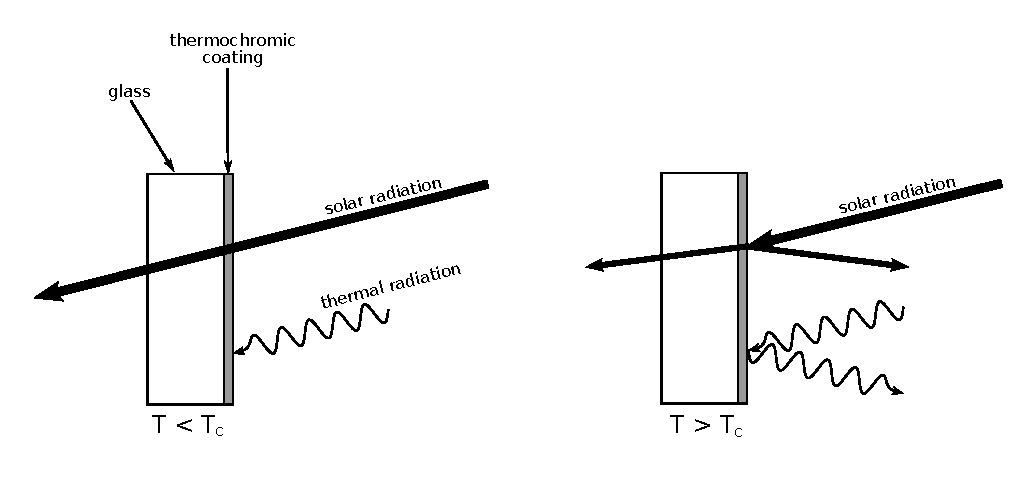
\includegraphics[width=0.5\textwidth]{Figures/TCcoating.pdf}
   \caption{Schematic demonstration of the application of thermochromic materials to advanced window glazing [8].
   In the article it is used as a pictorial representation of how vanadium(IV) oxide thin film will work as 
   an intelligent window. }
\end{figure}


\clearpage
\begin{thebibliography}{9}

      \bibitem{opticalProperties}
      D. Bedeaux, J. Vlieger, 
      \emph{Optical Properties of Surfaces}, 
      Imperial College Press, 
      London, 2001

      \bibitem{intelligentWindows}
      Parkin IP, Manning TD.
      \emph{Intelligent thermochromic windows}, 
      Journal of Chemical Education,
      London 2006;83(3):393. ?I DON'T KNOW WHAT 393 is!? what is it?


      \bibitem{TCcommercialProducts}
      White MA, LeBlanc M.
      \emph{Thermochromism in Commercial Products}, 
      Journal of Chemical Education,
      Canada, September 1999;76(9) ?IS THIS RIGHT? IS SOMETHING WRONG? DO I MISS SOMETHING?!

      \bibitem{TCqualitativeDescription}
      Hiltunen J, Silfsten P, Jaaskelainen T, Parkkinen JPS,
      \emph{A Qualitative Description of Thermochromism in Color Measurements}, 
      ???????????????,
      ???????????????
      
      %\bibitem{Kamalisarvestani2013}
      %Kamalisarvestani M, Saidur R, Mekhilef S, Javadi FS,
      %\emph{Performance, materials and coating technologies of thermochromic thin films on smart windows}, 
      %Renewaable and Sustainable Energy Reviews 26 (2013) 353-364 ???????/????????   Elsevier?
      %Kuala Lumpur, Malaysia 2013; ???????????+

\end{thebibliography}


%
\newpage
\section{\textbf{Book Notes}}
\section{Handbook of Optial Constants of Solids; Edward D. Palik}
Institute for physical Science and Technology, University of Maryland\\
Academic Press 1998, 1985.\\

\subsection{Bulk and thin-film effects; effective-medium theory; p.104}
\begin{itemize}
\item p. 105:\\
   In this discussion, we assume that the characteristic dimensions of the microstructure
   are large enough ($>/\sim 10-20 $Å) so that the individual regions retain essentially their bulk dielectric
   responses, but small ($>/\sim$ 0.1-0.2 $\lambda$) compared to the wavelength of light.
   Then, the macroscopic $\boldsymbol E$ and $\boldsymbol H$ fields of Maxwell's equations will not vary
   appreciably over any single region, and quasistatic theory can be used. This avoids complications
   due to scattering and retardation effects that are dominant in macroscopiccally inhomogeneous 
   systems \cite{Beckmann1968}.
   \\
   \\
   The dielectric functions is obtained from the macroscopic average electric field $\boldsymbol E$ and 
   polarization $\boldsymbol P$ according to
   \begin{align}
      \boldsymbol D &= \varepsilon \boldsymbol E = \boldsymbol E+ 4\pi \boldsymbol P \\
      \boldsymbol P &= \frac{1}{V} \sum q_i \Delta\! \boldsymbol{x_i},
   \end{align}
   where $\Delta \! \boldsymbol{x_i}$ is the displacement of the charge $q_i$ under the action of the 
   local field at $q_i$. It is the apperance of the volume normalizing factor in the latter equation
   that is responsible for the sensitivity of $\varepsilon$ to density.
   \item 
\end{itemize}

\begin{thebibliography}{9}
      \bibitem{Beckmann1968}
      Beckmann P.
      The depolarization of electromagnetic waves.
      Golem, Boulder, Colorado, 1968.

\end{thebibliography}


\subsection{Jensen B: The Quantum Extension of the Drude-Zener Theory in Polar Semiconductors; p.169-188}
p.169-170:\\
\textbf{Introduction}\\
The classical Drude model for the complex dielectric constant of a semi-conductor can be used to
extrct the mobility and the free-carrier density $n_e$ from an analysis of the reflectivity and transmittance
data in the ar infrared (1-4)=
      \cite{Palik1979, Holm1977,Perkowitz1971,Perkowitz1974,Fan1967}.
The dielectric constant $\varepsilon$ is the square of the complex refractive
index, which determines the optical properties of a given material. One has
\begin{align}
   \varepsilon = \varepsilon_1 - i \varepsilon_2 = N^2,
   \label{compEps}
\end{align}
were the real and imaginary parts of the complex  parts of the complex dielectric constant $\varepsilon_1$ 
and $\varepsilon_2$ are functions of the complex refractive index N as
\begin{align}
   N = n -i k
\end{align}
\begin{align}
   \varepsilon = n^2 - k^2
\end{align}
\begin{align}
   \varepsilon = 2nk = \frac{4\pi \sigma}{\omega}
   \label{imEps}
\end{align}
The choice of $n-ik$ rather than $n+ik$ is determiend by the original use of 
$\exp i(\omega t - \boldsymbol q \cdot \boldsymbol r)$ in the assumed plane-wave solution of
Maxwell's equations.
In Eqs \eqref{compEps}-\eqref{imEps}, $n$ is the real part of the complex refractive index, $k$
the imaginary part or extinction coefficient, and $\sigma$ the optical conductivity. The
absorption coefficient $\alpha$ is proportional to $\sigma$, to $\varepsilon_2$, and to $k$:
\begin{align}
   n\alpha = \frac{4 \pi \sigma}{c} = \frac{\omega}{c} \varepsilon_2
\end{align}
\begin{align}
   n\alpha =  = \frac{\omega}{c}k = \frac{1}{\delta}
\end{align}
The extinction coefficient k is essentially the ratio of the free-space wavelength of light of 
frequency $\omega$ to the skin depth $\delta$.\\
%
The Drude theory gives the free-carrier contribution to $\varepsilon_1$ and $\varepsilon_2$ in terms
of the plasma frequency $\bar\omega_p$ and the electron scattering time $\tau$ as
\begin{align}
   \varepsilon_1 &= \varepsilon_{\infty} \frac{1 - \bar\omega_p^2}{\omega^2 \eta}\\
   \label{eps1Drude}
\end{align}
\begin{align}
   \varepsilon_2 &= \frac{\omega_p^2}{\omega^2 \eta} \frac{ 1 }{ \omega \tau}
\end{align}
where $\varepsilon_{\infty}$ is the high-frequencylattice dielectric constant The reail and imaginary
parts of the complex refractive index are obtained from $\varepsilon_1$ and $\varepsilon_2$.
One has
\begin{align}
   \varepsilon &= \sqrt{\varepsilon_1^2 + \varepsilon_2^2} = n^2 + k^2, \\
   n = \sqrt{\frac{\varepsilon + \varepsilon_1}{2} },
   k = \frac{\epsilon_2}{2n} = \sqrt{ \frac{\varepsilon - \varepsilon_1}{2}}.
\end{align}
Experimentally, $n$ and $k$ are found from measurements of the reflectivity R of a bulk, opaque sample
and the transmittance T of a slab, which are given in terms of $n$ and $k$ as
\begin{align}
   R &= \frac{(n-1)^2 + k^2}{(n+1)^2 + k^2} \\
   R &= \frac{ (1-R)^2 e^{-2\omega k d / c} }{ (1-R)^2 e^{-4\omega k d / c} },
\end{align}
where $d$ is the sample thickness. For the slab multiple-reflection effects are averaged,
so that interface fringes are not resolved.
\\
\\
p.171:\\ In the far infrared, for photon energues small compared with $k_0 T$ ($k_0$ boltzmans const.)
and with the energy $\hbar \omega_Q$ of the phonon involved in the scatteering, the
quantum result reduces to the $\lambda^2$ dependenve given by the Drude Theory, and the quasi classical
Boltzmann transport equation (1-3). The departurs from the Drude theory
at high frequencies are associated mainly with $k$ rather than $n$, and hence,
the transmission is affected more than the reflectivity. The latter depends on
$k$ in the region of the reflectivity minimum, where $n \simeq 1$, but is determined 
essentially by $n$ over the region of the absorption spectrum for which $n > k$,
which is the region where departures from the Drude theory would occur.
\\
(...)
\\
The response of electrons to a driving field may be followed from the wuasi-classical
limit of small $\omega$ to the quantum limit that occurs when $\hbar \omega$ is no longer small
compared with characteristic energies of the system. In this case, a generalized Boltzmann equation
is obtained that reduces to the quasi-classical Boltzmann transmport equation when the electron wave 
vector $q$ tends to zero and $\omega$ is small (14-17)=
\cite{Jensen1975,Price1966,Argyres1961,Kohn1958}
. When $\omega$ is appreciable, one obtaines,
under certain conditions, a solution of the Boltzmann equation in terms of a frequency-dependent
relaxation time. This relaxation rate, which has been tabulated as a function of frequency and 
carrier concentration for various materials (18-20)=
\cite{Jensen1977,Jensen1979,Jensen1981}
, can be used in the usual expression of the 
classical Drude theory to obtain the quantum result. In particular, the low-
frequency $\hbar\omega \simeq k_0T$ limit gives a good estimate for the dc mobility as a function
of carrier concentration. At high frequencies, in lightly doped materials in which
polar scattering dominates, $n\alpha$ is proportional to $\lambda^3$ and $\varepsilon_2$ and $k$
are proportional to $\lambda^4$ rather than $\lambda^3$. The real part of the dielectric constant
is givn approximately by the Drude-theory expression and $n \simeq \sqrt{\varepsilon_{\infty}}$
for $\bar\omega_p \ll \omega \ll G/\hbar$, where $G/\hbar$ is the frequency of the fundamental absorption
edge and $G$ is the direct-band-gap energy of the semiconductor. As $\omega$ approaches $G/\hbar$ there
is a small quantum-mechanical correction to $\varepsilon_1$ and hence to $n$.
A summary of the results of the quantum theory is given in Section II.
\\
\\
p.176:\\
\textbf{Comparison with experimental data}\\
A calculation of $\varepsilon_1$ appropriate to electrons in polar semiconductors with the
band structure of the Kane theory and based on the quantum density-matrix equation of motion yields a 
high frequency modification to Eq.\eqref{eps1Drude}. 
For $\omega \tau \gg 1$ and $X < 0.1$, ($X = \hbar \omega/G$) one obtains (18,22)
\begin{align}
   \varepsilon_1 &= \Bigg[ \frac{\varepsilon_{\infty}}{1 - X} \Bigg]\big[ 1 - (X/\varepsilon_{\infty}) - \bar\omega_p^2/\omega^2 \big] \\
                &= \Bigg[ \frac{\varepsilon_{\infty}}{1 - X} \Bigg]\big[ 1 - \bar\omega_p^2/\omega^2 \big] \\
                &= \varepsilon_{\infty}(1 - \bar\omega_p^2/\omega^2), \:\:\:\:\: X \ll 1
\end{align}
We note that $1/\varepsilon_{\infty} <\sim$ 0.1 and hence $X/\varepsilon \ll 1$, for compounds we 
consider, and this term can be neglected. In the limit $X \ll 1$, the quasi-classical high-frequency
Drude result is recovered, as required. For $X \sim 0.1$, there is a high-frequency correction given by
Eq.(some equation), which is used to calculate the numerical values of $\varepsilon_1 = n^2 - k^2$.
The major modification of the classical result is dispersion in $n$ as one approaches the fundamental
absorption edge \cite{Jensen1983}.


\begin{thebibliography}{9}
      \bibitem{Palik1979}
       Palik ED, Hold RT.
       Nondestructire evaluation of semiconductor materials and devices.
       Plenum 1979 (Chap. 7) 
      \bibitem{Holm1977}
         Holm RT, Gibson, Palik ED, 
         J. Appl.Phys. 48,212 (1977)
      \bibitem{Perkowitz1971}
         Perkowitz S. J.Phys.Chem.Solids 32, 2267 (1971)
      \bibitem{Perkowitz1974}
         Perkowitz S, Thorland RH, Phys.Rev. B9, 545 (1974)
      \bibitem{Fan1967}
         Fan HY.
         Semiconductors and semimetals.
         (R.K. Willardson and A.C. Beer eds.),
         Vol.3, Academic Press, New York 1067

      \bibitem{Jensen1975}
         Jensen B. Ann. Phys. 95,229 (1975).
      \bibitem{Price1966}
         Price PJ. IBM J. Res. Dev. 10,395(1966)
      \bibitem{Argyres1961}
         Argyres PN, J. Phys.Chem.Solids 19, 66 (1961)
      \bibitem{Kohn1958}
         Kohn W, Luttinger JM.
         Phys. Rev. 108, 590 (1957)
         Kohn W, Luttinger JM.
         Phys.Rev.109,1892(1958)

      \bibitem{Jensen1977}
         Jensen B. Phys. StatusSolidi. 86, 291 (1978);
         Jensen B. SolidState commun. 24, 853 (1977)
      \bibitem{Jensen1979}
         Jensen B. J. Appl Phys. 50, 5800 (1979)
      \bibitem{Jensen1981}
         Jensen B.
         Laser Induced damage in optical materials; 1980 (H.E. Bennet, A.J. Glass, A.H. Guenther,
         and B.D.Newman, eds.), p.416, National bureau of standards special
         publication 620, Boulder, Colorado, 1981.

      \bibitem{Jensen1983}
         Jensen B, IEEE J. 
         Quantum Electron. QE-18, 1361 (1982); 
         %
         Jensen B, Torabi A, IEEE J.Quantum Electron. QE-19, 448-457,877-882,1362-1365 (1983);
         %
         Jensen N, Torabi A, J.Appl.Phys. 54,2030-2035,3623-3625,5945-5949 (1983).
\end{thebibliography}





\subsection{Shashanka S. Mitra \\
Optical properties of nonmetallic solids for photon energies below the fundamental band gap}
Department of electrical engineering, University of Rhode Island.
\\
\\
p.263-267:\\
\textbf{Infrared Dispersion by plasmons}\\
In the preceeding discussion of absorption of infrared radiation by phonons in a solid, it was tacitly
assumed that the solid was an insulator. This assumption does not hold well for a narrow--gap semiconductor at
ordinary temperatures or for a doped semiconductor with a partially filled conduction or valence band.
The collective excitation of this free-carrier electron gas(plasma) in such a crystal will modify the
infrared absorption by phonons, as discussed earlier. The dispersion mechanism through which electromagnetic
radiation interacts with a solid should include the contribution of free-charge carriers in solids for which
their numbers are significant, in addition to contributions from bound electrons and phonons.
The dielectric response function of such a solid can now be written as 
\begin{align}
   \varepsilon = 1 + 4\pi(\chi_{BE} + \chi_L + \chi_{FC}),
\end{align}
where $\chi_{BE}, \chi_L$ and $\chi_{FC}$, respectively represent the bound electron,lattice,and
free-carrier contributions to the electrical susceptibility. For the spectral region of interest, we
are not concerned with teh bound-electron dispersion; thus this term, as usual, will be 
represented by a dispersion-free, high-frequency dielectric-constant term
\begin{align}
   \varepsilon_{\infty} = 1 + 4\pi \chi_{BE}.
\end{align}
An approximate expression for the dielectric response function for a free-electron gas in a solid can be
obtained from the classical Drude model in which a free electron of effective mass $m*$ and charge $e$
is displaced by an amound $\boldsymbol x$ as a result of interaction with the electric field 
$\boldsymbol E$, with the equation of motion
\begin{align}
   m* \ddot{\boldsymbol x} + m* \gamma \dot{\boldsymbol x} = e \boldsymbol E_0 e^{-i\omega t}
\end{align}
The damping term proportional to the velocity obviously represents the electron-phonon scattering in 
a phenomenological manner. Solving for $\boldsymbol x$, one obtains
\begin{align}
   \boldsymbol x = -e \boldsymbol E /m* \omega (\omega + i \gamma)
\end{align}
The polarization, defined as the electric-dipole moment per unit volume, is given by
\begin{align}
   \boldsymbol P = Ne \boldsymbol x,
\end{align}
where N is the carrier concentration. Recalling that 
\begin{align}
   \boldsymbol P =  \big[ (\varepsilon - 1)/ 4\pi \big] \boldsymbol E,
\end{align}
one readily obtains
\begin{align}
   \varepsilon_{FC} = \varepsilon_{\infty} - \frac{4 \pi N e^2}{m*\omega(\omega + i \gamma)}
\end{align}
for the dielectric response function due to a single-component plasma. In terms of the plasma frequency
defined as 
\begin{align}
   \omega_p = \sqrt{\frac{4\pi N e^2}{\varepsilon_{\infty} m*}}
\end{align}
$\varepsilon_{FC}$ becomes
\begin{align}
   \varepsilon_{FC} = \varepsilon_{\infty} \big[ 1 - \big(\omega_p^2/\omega(\omega + i \gamma)\big)\big].
\end{align}
For a number of semiconductors there exists a region of the infrared spectrum in which the free-carrier 
contributions dominates, and both the bound electron and lattice contributions to dielectric response
function are negligible. For a semiconductor, such a situation prevails in a region of the infrared
spectrum in which $\omega_g \ll \omega_p \ll \omega_{TO}$, where $\hbar \omega_g$ is the
electronic band gap. The analysis of optical response is also smpler in a region in which the reflection


\begin{thebibliography}{9}
      \bibitem{yy}
\end{thebibliography}

\newpage
\section{\textbf{Optical Properties of Surfaces Notes}}
\begin{itemize}
\item $\rho$ is the number of island per unit of surface area.
\item $\alpha_{\parallel}^{10}$: (averge) parallel quadrupole polarizability \\
   $\alpha_{\perp}^{10}$: (average) normal quadrupole polarizability
   \item 
   \begin{align}
      \tau = -\rho \alpha_{\parallel}^{10} \:\:\:\text{ and }\:\:\: \delta = -\rho [\alpha_{\perp}^{10} + \alpha_{\parallel}^{10} ]/\varepsilon_a
   \end{align}
   $\varepsilon_a$ is the ambient/surrounding dielectric constant.

   \item an extremely important difference between an interface and the bulk of the adjacent phases is the
   inherent asymmetry of the interface in its responce to fields normal to the surface or parallel
   to the interface. This is eminently clear for a thin metal film between two dielectric media.
   If one applies an electric field along the film this results in a current while 
   an electric field normal to the film does not lead to a current. (p.7)

   \item excess quantities which not affect the boundary conditions have no relevance for the reflection
   and transmission of light by the interface.

   \item The resistance of the sublayers are put in series and add up for an electric field perpendicular
   to the surface. This is very different from the case described above for an electric field parallel
   to the layer where the conductivities of the sublayers were put in parallel. 
   \\
   \\
   If the electric field is parallel to teh layer, one finds an important contribution from the layer if its 
   conductivity is large compared to the surrounding medium. \\
   For a field orthogonal to the layer, however, one finds an important contribution if the conductivity
   of the layer is much smaller than the conductivity of the surrounding medium. It is this very characteristic
   difference in the response of the layer to fields orthogonal and parallel to teh layer which is the
   origin of many of the interesting electromagnetic properties of the layer. (p.10)

   \item If the electric field is parallel to the layer the dielectric constants of the sub-layers are so
   to say put in parallel. If the elextric field is normal to the layer, however, they are put in series.
   Furthermore one finds that, if the dielectric constant of the layer is much larger than the dielectric
   constants of the surrounding homogeneous media, the constitutive coefficient $\gamma_e$ is much smaller 
   than the coefficient $\beta_e$ and dominates the behaviour of the layer. IF the dielectric constant
   of the layer is much smaller than the dielectric constants of the surrounding homogeneous media,
   the constitutive coefficient $\beta_e$ is much larger than the coefficient $\gamma_e$ and dominates the
   behaviour of the layer. It is again this very characteristic difference in the response of the layer
   in the directions orthogonal and parallel to the layer which is the origin of many of the
   interesting electromagnetic properties of the layer. (p.13)

\item the jump in the extrapolated fields are given in terms of the total excess of 
$D_{ex,\parallel}$,$E_{ex,z}$,$B_{ex,\parallel}$,$H_{ex,z}$,$I_{ex,\parallel}$ and $\rho_{ex}$.
Notice that it is however not affected by the total excesses of
$D_{ex,z}$,$E_{ex,\parallel}$,$B_{ex,z}$,$H_{ex,\parallel}$,$I_{ex,z}$ and $\rho_{ex}$;
these total excesses tehrefore have no effect on the reflection and transmission
amplitudes and may as such be neglected in the descripttion of the optical properties of the 
interface.(?I think this is for $k_z = 0$?). (p.16)

\item p.21 - 72. NOT READ

\item If one consider a single island surrounded by the ambient the electro-magetic response may be
characterized by dipole, quadrupole and higher order multipole polarizabilities. If this particle
is brought close to the substrate the multipole polarizabilities are modified, due to an 
induced charge distribution on the surface of the substrate, and become dependent on the distance to
the substate. (p.73)
\item neighboring island interaction also changes the polarizabilities of the island and result in 
polarizabilities parallel and othogonal to hte surface which are unequal, even if the islands are spherical.
As a consequence the film is anisotropic in its reaction to fields parallel versus fields normal to the 
surface. Further contribution to this anisotropy is achieved if the particle is not symmetric.
(p.73)

\item The resulting dipole polarizabilities of the islands, parallel and orthogonal to the
surface , are directly related to teh constitutive coefficients $\gamma_e$ and $\beta_e$, respectively.
The susceptibilities $\delta_e$ and $\tau$ account for the fact that the dipoles are situated at a
finite distance from the surface of the substrate. It follows in the context of the polarizable
dipole model that $\beta_e$ and $\gamma_e$ are proportional to the typical diameter of the islands times the
coverage. The coverage is the surface area of the particles as viewed from above divided by
the total surface area. For identical spheres the coverage is equal to $\pi r^2 \cdot N_{islands}/A$.
Furthermore it follows that $\delta_e$ and $\tau$ are proportional to the diameter times the distance
of the center of the islands to the substrate times the coverage.\\
In general, and not only in the polarizable dipole model, one may in fact use the ratio of the coefficients
$\delta_e$ and $\tau$ with the coefficients $\gamma_e$ and $\beta_e$ as a rough measure for the distance
of the center of the islands to the substrate. (p.74) 

\item  the first term ($A_{lm}$ term) is due to sources located in the region r < a.
The second term ($B_{lm}$ term) is due to sources in the region r > b and may be identified
as the incident field due to external sources. The first term is due to the charge distribution induced
in the island. The island has no net charge $\rightarrow$ the l = 0 contribution in the first term
is zero. $A_{lm}$ gives a contribution to the potential which decaus as $r^{-l-1}$, and may be
identified (apart from a numerical constant) as an amplitude of the $l$'th order mutlipole field. 
\\
The amplitude of these multipole fields are given in terms of the amplitudes of the 
incident field using a polarizability matrix:
\begin{align}
A_{lm} = - \sum\limits^{'}_{l',m'} \alpha_{lm,l'm'} B_{l'm'} \:\:\:\:\text{ for } l \neq 0
\end{align}
where the prime over sum indicates that $l' \neq 0$.
   \begin{itemize}
      \item polarizable dipole model:  all amplitudes with $l$ and $l' \neq 1$ is set to zero.
      \item polarizable quadrupole model: all amplitudes with $l$ or $l' > 2$ is set to zero.
   \end{itemize}
   (p.79)

\item s. 80 viser en del intuitiv forklaring av hvordan polariseringen påvirker feltet i øvre og nedre
medium. Kan hjepe å forstå hvordan de første $A_{lm}$ amplitudene representerer dipolbidraget.
\item For particles with symmetry axis normal to the surface of the substrate ($A$ characterizses the strength
of the reflected dipole):
\begin{align}
&\alpha_{\parallel}(0) = [1 + A \alpha_{\parallel}]^{-1} \alpha_{\parallel} \\
&\alpha_{\perp}(0) = [1 + 2 A \alpha_{\perp}]^{-1} \alpha_{\perp}
\end{align}
If there are two two different polarizabilities parallel to teh surface the above equation is valid for 
both of them. Furthermore, regarding the anisotropy in the interaction with the substrate, even
if the particle is spherical, so that $\alpha_{\parallel} = \alpha_{\perp}$, the different response
to fields along the surface and normal to the surface results in $\alpha_{\parallel}(0) \neq \alpha_{\perp}(0)$.
(p.81).
\\
\\
If one covers the substrate with a low density of identical islands, which have a rotational symmetry
around the normal of the surface, one finds for the first order interfacial susceptibilities
\begin{align}
\gamma_e(d) = \rho \alpha_{\parallel}(0) = \rho[1 + A \alpha_{\parallel}]^{-1} \alpha_{\parallel}\\
\beta(d)_e = \rho \varepsilon_a^{-2}\alpha_{\perp}(0) = \rho \varepsilon_a^{-2}[1 + 2 A \alpha_{\perp}]^{-1} \alpha_{\perp},
\end{align}
where $\rho$ is the number of particles per unit of surface area. The argument $d$ indicates
that the location of the dividing surface is chosen to be the $z=d$ surface, which in this case
coincides with the surface of the substrate. One important thing: in writing these formulae the polarization
due to the dipoles is in fact taken to be located at the surface of the substrate. The origin of $tau$ and
$\delta_e$ is related to a proper choice of this location.

\item The reason, that it is also in the dipole model important to take 
finite values for $\delta_e$ and $\tau$, is related to the occurence of phase factors. Light reflected from
the film can either be reflected directly from the island film or be transmitted and subsequently
reflected by the surface of the substrate. It is clear that the phase difference between these
two contributions can be important. The analysis on p. 83 and the resulting finite value of 
$\delta_e$ and $\tau$ account for the phase differences between the actual location of the islands
and the surface of the substrate to linear order. (p.83)
\item $\delta_e$ and $\tau$ have relatively small modification of the optical properties, but contain 
nevertheless interesting new information. The coefficients $\gamma_e$ and $\beta_e$, which usually
have a much larger influence, are a measure of the amount of material deposited on the surface 
of the substrate. They are therefore a measure of what on usually calls teh weight thickness.

\item (p.95)\\
   Incident e field $ \boldsymbol E_0$ and the corresponding potential 
$\psi_0(\boldsymbol r) = - \boldsymbol E_0 \cdot \boldsymbol r$ is given on .

\item Appendix A (p. 106): The derivation of the surface constitutive coefficients $\gamma_e(d)$ and 
   $\beta_e(d)$. for an identical particle, island film, in the low density limit 
   \\
   \\
   Instead of dipoles, small dielectric spheres are considered, 
   located a distance $d \gg R$ above the substrate (substrate is located at $z = d$).
   Excess fields are introduced and the total field in the ambient is the sum of the external field,
   the dipole fields of the spheres (with centers in $(\boldsymbol R_{i,\parallel},0)$) and the
   image dipoles (with centers in $(\boldsymbol R_{i,\parallel},2d)$).

\item (p.117)\\
   When the islands are broughth close to the substrate, one must also account for the 
   modification of their dipole and quadrupole polarizabilities due to the interaction with higher order 
   multipoles in the substrate. It is sufficient to calculate only the modification of these 
   polarizabilities, as long as one is interested in the constitutive coefficients $\gamma_e$, $\beta_e$,
   $\delta_e$ and $\tau$. 
\item (p.118)\\
   The dipole and the quadrupole approximation is in general inadequate for islands which are flat, i.e.
   islands for which teh distance of the center to the surface of the substrate is smaller than 30\% of
   the linear diameter along teh surface. 
   
\item p.173

\item p.204\\
   (I think this is for the dipole + quadrupole expansion.. maybe) \\
   The calculations were done for scaled densities $\hat \rho \equiv \rho(2R)^2 = (2R/L)^2 = (2\hat R)^2$ of
   0 (no interaction), 0.2, 0.4, and 0.8. L is the lattice cosntant and $\hat R \equiv R/L$. The reason
   to go to a higher order in the multipole expansion in the interaction with the substrate is that,
   close to touching the substrate, the higher order multipoles start to give corrections of about 5 to 10\%.
   As is analyzed in great detail by Haarmans and Bedeaux (49),\textbf{higher order multipole corrections 
   for the interaction along the substrate become important for $\hat \rho > 0.9$. They use as density
   parameter the coverrage, which is equal to $(\pi/4)\hat \rho$ for the square array.}
   (...) The interaction along the substrate has a substantial effect on the size of the polarizabilities and 
   the resulting constitutive coefficients. The polarizability along the substrate approximately doubles 
   from $\hat \rho = 0$ to 0.8 (?for triangular lattice?), while the polarizability normal to the surface
   decreases by a factor of 2. The resonance frequency shifts a little bit down for the polarizability
   parallel and up for the polariability normal to the surface. The contributions due to the 
   quadrupole polarizabilities to the coefficients $\hat \delta_e$ and $\hat \tau$ are small compared to
   the contributions due to the dipole polarizabilities. \\
   \\
   p.209\\
   These coefficient are therefore mainly due to the shift of the induced dipole to the surface of 
   the substrate.
\item p.209-210.\\
   \textbf{Here (also something about square lattice), they talk about that the distance between the
   islands must be so far apart to give reasonable results.}It also seems like they're saying that
the polarizabilities and constitutive coefficients of OBLATE SPHEROIDS do not depend very much on the
coverage. The reason is that the center of the OBLATE SPHEROIDS remain relatively far apart, even for high
densitites. \\
For PROLATE SPHEROIDS the dependence on the coverage becomes dramatic, reason being that they approach each
other for higher coverage to distances smaller than the long axis. It is to be expected that these results
are unreliable for the combination of a high density and a small axial ratio\\
\\
If one would set a criterium that the distance between the particles should be larger than half the 
long axis, one finds that for densities 0.0,0.2,0.4 and 0.8 the maximum values of 1/(1+AR) are
1.00,0.69,0.61 and 0.53 respectively. It follows that all the new maxima appearing for larger values of 
$\hat rho$ and 1/(1+AR) are outside the range of reliability of the dipole approximation for the 
interaction along the substrate. Since the shape of the particles in island films is usually oblate
rather than prolate, the dipole approximation to describe the interaction between the particles 
will in practice suffice.

\end{itemize}

\newpage
\section{Color notes from wikipedia}
\begin{itemize}
\item Humans tend to percieve light within the green parts of the spectrum as brighter than
red or blue light of equal power. The luminosity function that describes the percieved brightnesses
of different wavelengths is thus roughly anagagous to the spectral sensity of M cones.
\item \textbf{With three color apperance parameters- colorfulness(or chroma or saturation), lightness 
   (or brightness), and hue, any color can be described.}
\item \textbf{Hue} is one of the main properties of a color. There are six (unique) hues: 
   red, orange, yellow, green, blue and purple. ?Hue is described as the degree to which
   a stimulus can be described as similar to or different from stimuli that are described by the unique
   hues?
\item \textbf{Colorfulness} is the visual sensation according to which the percieved color of an area appears
   to be more or less chromatic. A highly colorful stimulus is vivid and intense, while a less colorful
   stimulus appears more muted, closer to gray. With no colorfulness at all, a color is a
   "neutral" gray (an image with no colorfulness in any of its color is called grayscale).
\item \textbf{Chroma} is the colorfulness relative to the brightness of a similarly illuminated area that 
   appears to be white or highly transmitting. (therefore) Chroma should not be confused with colorfulness!
\item Saturation is the colorfulness of a color relative to its own brightness.
\item \textbf{Lightness} (aka value or tone) is a representation of variation in the perception of
   a color or color space's brightness. Lightness is a relative term. Lightness means Brightness
   of an area judged relative to the brightness of a similarly illuminated area that appears to be white 
   or highly transmitting. Lightness should not be confused with brightness.
\item \textbf{Brightness} is an attribute of visual perception in which a source appears
   to be radiating or reflecting light. Brightness is the perception elicited y the luminance 
   (how much luminous power will be detected by an eye looking at e.g. a surface from a particluar angle
   of view) of a visual target. This is a sibjective property of an object being observed and 
   one of the color apperance parameters of color apperance models. Brightness refers to an
   absolute term and should not be confused with Lightness.
   \\
   \\
   In RGB color space, brightness can be thought of as the arithmetic mean $\mu$ of the red, green and blue
   color coordinates (although some of the three components make the light seem brighter than others).
   \begin{align}
      \mu = \frac{R + G + B}{3}
   \end{align}
   Brightness is also a color coordinate in the HSB or HSV color space (Hue, Saturation, and Brightness/Value).
\end{itemize}

\newpage
\section{Color notes regarding \textsc{ColorPy}}
source: http://markkness.net/colorpy/ColorPy.html
\\
\\
How I installed it:
\begin{itemize}
   \item download zipped folder and unzip it using:\\
      gunzip -c colorpy-0.1.0.tar.gz | tar xf
      \\
      \\
      The unzipped folder can be put anywhere (doesn't matter). Go to it (cd path/colorpy-0.1.0).
      Personally, I ran the following command (don't know if you need administrator privileges, 
      but it seemed like it was required: \\
      sudo python setup.py install 
      \\
      \\
      After than I made a folder ''TEST'', went into it, started python and ran the following commands to
      test that the program/module worked correctly:\\
      \# running test cases: \\
      import colorpy.test\\
      colorpy.test.test()\\
      \\
      \# generate sample figures: \\
      import colopy.figures\\
      colorpy.figures.figures()\\
      \\
\end{itemize}
Fundamentals:
\begin{itemize}
   \item \textsc{ColorPy} generally uses wavelengths measured in nanometers, otherwise typical metric
      units are used.
   \item The description of the spectra, \textsc{ColorPy} uses two-dimensional NumPy arrays:
      column 1: wavelength[nm], column 2: light intensity at the wavelength.
   \item Color values are represented as three-component NumPy vectors (1D-arrays). Typically, these are 
      vectors of floats, except for irgb colors, which are arrays of integers in the range 0-255.
   \item \textsc{ColorPy} can provide a blank spectrum array, via colorpy.ciexyx.empty\_spectrum(),
      which have rows for each wavelength from 360nm to 830nm, at 1nm increments.
   \item To go from the light spectra to a color (a 3D quantity), we use a set of three matching functions
      \begin{align}
         X = \int I(\lambda) \cdot C\!I\!E\!-\!\!X(\lambda) d\!\lambda\\
         Y = \int I(\lambda) \cdot C\!I\!E\!-\!\!Y(\lambda) d\!\lambda\\
         Z = \int I(\lambda) \cdot C\!I\!E\!-\!\!Z(\lambda) d\!\lambda
      \end{align}
   \item The Y-matching function corresponds exactly to the luminous efficiency of the eye - the eye's
      response to light of constant luminance (these facts are some of the reasons that make this 
      particular ser of matching functions so useful).
   \item Rescaling XYZ so that their sum is 1.0, we get the values xyz (i.e. $x + y + z = 1$).
      The chromaticity is given by x and y (z can be recontructed as $z = 1.0 - x - y$). 
      It is also common to specify colors with the chromaticity (x,y) , as well as the total
      brightness (Y). Occasionally, one also wants to scale XYZ colors so that the resulting Y value is 1.0.

   \item Here are some 'constructor'-like functions for creating the colors (e.g.XYZ), which are 
      three-compontent vectors.
\begin{lstlisting}[style=FormattedNumber, language=python, frame=none]
   colorpy.colormodels.xyz_color(x,y,z=None)
   colorpy.colormodels.xyz_normalize(xyz)
   colorpy.colormodels.xyz_color_from_xyY(x,y,Y)
   colorpy.colormodels.xyz_normalize_Y1(xyz)
\end{lstlisting}
   Note that color types are generally specified in ColorPy with lower case letters, as this is more 
   readable. The user must keep track of the particular normalization that applies in each situation.
\end{itemize}
Fundamentals - converting XYZ colors to RGB colors which we can draw on the computer:
\begin{itemize}
   \item To convert we can use
\begin{lstlisting}[style=FormattedNumber, language=python, frame=none]
   # Here, xyz is the XYZ color vector:
   colorpy.colormodels.irgb_from_xyz(xyz) # Returns [int,int,int] (int in [0,255])
   colorpy.colormodels.irgb_string_from_xyz(xyz) # Returns hex string, e.g. '#FF0000' for red.
\end{lstlisting}

\item 
Note that there are several subtleties and approximations which are important to understand
what is happening in the code above.
   \begin{itemize}
      \item the XYZ color is converted to a linear RGB color(represented as floats in the range 0.0-1.0),
         meaning that the light intensity is 
         proportional to the numerical color values, and is done by a 3x3 element array. The values
         of the array depends on physical display in question, so the conversion matric cannot apply to 
         all displays/monitors. Fortunately, we can assume a specification of monitor chromaticities
         (which are a part of the sRGB standard) which are likely to be close to most displays. 
         \textsc{ColorPy}
         uses this assumption by default, although you can change the assumed monitor chromaticities to nearly
         anything you like.
      \item The RGB colors can be out of range: 
         \begin{enumerate}
            \item greater than 1.0, meaning the color is too bright for the display. 
            \item negative value, meaning that the color is too saturated and vivid for the display.
         \end{enumerate}
         To put these values between 0.0-1.0 that can actually be displayed is known as color clipping:
         The first is solved by rescaling such that the maximum value is 1.0, making the 
         color less bright without changing the chromaticity. The second change required some change in
         chromaticity. By default,  \textsc{ColorPy} adds just enough white to the color to make all the
         components non-negative. (There is also the potential to develop better clipping functions.)
      \item The next subtlety is that the intensity of colors on the display is not simply
         proportional to the color values given to the hardware. This situation is known as 
         the 'gamma corretion'. We rely on the sRGB standard what to do. The standard assumes a 
         physical 'gamma' exponent of about 2.2., and \textsc{ColorPy} applies this correction by default
         (can be changed if you like).
      \item The final step is to convert the RGB components from 0.0-1.0 to 0-255 (done with simple scaling
         and rounding).
   \end{itemize}
\item Summarizing these conversions:
   \begin{itemize}
      \item The function
\begin{lstlisting}[style=FormattedNumber, language=python, frame=none]
   colorpy.colormodels.rgb_from_xyz(xyz)
\end{lstlisting}
      converts an XYZ color to linear RGB color in range 0.0-1.0. Can be out of range or negative, and
      can not be directly passed to drawing functions.
   \item The function
\begin{lstlisting}[style=FormattedNumber, language=python, frame=none]
   colorpy.colormodels.irgb_from_rgb(rgb)
\end{lstlisting}
      converts a linear RGB in the range 0.0-1.0 to a displayable irgb color, definitely in the range 
      0-255. Color clipping may be applied (intensity and chromaticity), and gamma correction is 
      accounted for. This result can be passed to drawing functions.
   \end{itemize}

\item To plot the visible spectrum:
\begin{lstlisting}[style=FormattedNumber, language=python, frame=none]
   colorpy.plots.visible_spectrum_plot()
\end{lstlisting}
To plot the RGB values for the pure spectral lines (?or visible spectrum?), use:
\begin{lstlisting}[style=FormattedNumber, language=python, frame=none]
   colorpy.plots.color_vs_param_plot(param_list, rgb_colors, title, 
      filename, tight=False, plotfunc=pylab.plot, xlabel='param', ylabel='RGB Color')
\end{lstlisting}
In this case, the parameter list is wavelength and we also include a list of RGB colors. These must be of
the same size. This is a very handy function, useful for many other plots besides this one.

\item CIE chromaticity diagram of the visible gamut:
\begin{lstlisting}[style=FormattedNumber, language=python, frame=none]
   colorpy.plots.shark_fin_plot()
\end{lstlisting}

\item 'Patch' plot:
\begin{lstlisting}[style=FormattedNumber, language=python, frame=none]
   colorpy.plots.xyz_patch_plot(xyz_colors, color_names, 
      title, filename, patch_gap=0.05, num_across=6)
\end{lstlisting}
\texttt{xyz\_colors} and \texttt{color\_names} are two lists (which must be of same size).
You can pass 'None' for the second list to skip the labels. (There are also optional arguments to fine-tune
the size and arrangement of the patches.) \\
There is also a similar function:
\begin{lstlisting}[style=FormattedNumber, language=python, frame=none]
   colorpy.plots.rgb_patch_plot()
\end{lstlisting}
when you have known RGB values that you want to draw.

\item To plot spectrums like black body spectrums, use
\begin{lstlisting}[style=FormattedNumber, language=python, frame=none]
   colopy.plots.spectrum_plot(spectrum,title,filename,xlabel,ylabel)
\end{lstlisting}
Here, \texttt{spectrum} is a numpy array.
\\
\\
\textsc{ColorPy} allows us to plot the resulting color vs. temperature, while also showing a plot
of the rgb color values:
\begin{lstlisting}[style=FormattedNumber, language=python, frame=none]
   colopy.plots.color_vs_param_plot(param_list, rgb_colors, 
      title, filename, tight, plotfunc, xlabel, ylabel)
\end{lstlisting}
The arguments \texttt{tight, plotfunc, xlabel, ylabel} are optional. (In the example, he used
tight=True, plotfunc=pylab.semilogy to obtain the semilog plot, which is needed for the very large range
of color values covered).
\end{itemize}

\end{document}


